%%%%%%%%%%%%%%%%%%%%%%%%%%%%%%%%%%%%%%%%%%%%%%%%%%%%%%%%%%%%%%%%%%%%%%%%%%
%                                                                         %
%			TESI LAUREA TRIENNALE - INFORMATICA MUSICALE                  %                                            %																		  %
%			______________                                                %
%                                                                      	  %
%			AUTORE: Albanese Mirko                                        %
%                                                                         % 
%			Ultima revisione: ----                                        %
%                                                                         %
%%%%%%%%%%%%%%%%%%%%%%%%%%%%%%%%%%%%%%%%%%%%%%%%%%%%%%%%%%%%%%%%%%%%%%%%%%%

\documentclass[12pt]{report}

%
%			PREAMBOLO


\usepackage[a4paper]{geometry}
\usepackage{amssymb,amsmath,amsthm}
\usepackage{graphicx}
\usepackage{graphicx, subfigure} 
\usepackage{url}
\usepackage{hyperref}
\usepackage{epsfig}
\usepackage[italian]{babel}
\usepackage{tesi}
 \usepackage[a-1b]{pdfx}

\setcounter{tocdepth}{4}

% per le accentate
\usepackage[utf8]{inputenc}

\newtheorem{myteor}{Teorema}[section]
\newenvironment{teor}{\begin{myteor}\sl}{\end{myteor}}

\begin{document}

\pagenumbering{gobble}
\begin{center}
	{\LARGE \uppercase{Universit\`a degli Studi di Milano}}\\
	\uppercase{Facolt\`a di Scienze e Tecnologie}\\
	\vskip 0.6 cm
	\centerline{
\includegraphics[height=20mm]{logo}}
	\vskip 0.4 cm
	\uppercase{Corso di Laurea triennale in Informatica Musicale}
\end{center}

\vfill
\vskip 1.5 cm

\begin{center}
	{\Large\uppercase\expandafter{Analisi del comportamento della doppia incisione di chitarre e voci in una produzione musicale}}
\end{center}


\vfill
\vskip 3 cm

\begin{tabular}{ll}
	{\large Relatore:} & Goffredo Haus\\
	{\large Correlatore Interno:} & Giorgio Presti\\
	{\large Correlatore Esterno:} & Disi Melotti\\
\end{tabular}

\vfill
\vskip 0.5 cm

\begin{tabular}{l}
	\hspace{9cm}{\large Tesi di Laurea di:}\\
	\hspace{9cm}{\large Mirko Albanese}\\
	\hspace{9cm}{\large Matr. Nr. 828180}\\
\end{tabular}

\vfill
\vskip 2 cm

\begin{center}
	\sc anno accademico 2017-2018
\end{center}\vskip.5in

\prefacesection{Prefazione}
In questo elaborato viene descritto il progetto effettuato presso ~IK Multimedia (\url{http://www.ikmultimedia.com/}), azienda di produzione software e hardware nel campo musicale con sede a Modena (Italia). Il progetto svolto prende in considerazione una tecnica utilizzata nelle produzioni musicali, la {\itshape doppia incisione}.\\
La doppia incisione è una tecnica molto usata da diversi produttori discografici fondamentale per garantire una notevole resa stereofonica.\\
Durante il processo di registrazione di una produzione musicale si usa di solito incidere le chitarre e altri strumenti eseguendo due, quattro, otto volte la medesima parte musicale per poi ripartire a proprio piacimento le singole tracce nell'immagine stereo in modo da avvolgere l'ascoltatore. In questo elaborato si prenderanno in considerazione solamente una coppia ripartita, una destra e una a sinistra, nella suddetta immagine.\\
Lo scopo del progetto è di estrarre le differenze di {\itshape Dinamica}, {\itshape Frequenza}, {\itshape Timbro} e {\itshape Tempo} tra le due tracce in esame utilizzando l'ambiente e il linguaggio per il calcolo numerico {\itshape MATLAB}.\\

%\section*{Organizzazione della tesi}
\label{organizzazione}
La tesi è organizzata come segue:
\begin{itemize}
\item nel Capitolo \ref{cap1} verrà effettuata un'introduzione sul progetto svolto presso IK Multimedia andando a descrivere gli obiettivi e le finalità.
\item nel Capitolo \ref{cap2} verrà fornita una breve panoramica sui fondamenti teorici utili alla comprensione degli argomenti esposti.
\item nel Capitolo \ref{cap3} verrà presentata quella che è lo stato dell'arte per l'estrazione della dinamica, l'estrazione del contenuto frequenziale (tracciamento delle armoniche) utilizzando e confrontando due modelli di implementazione (interpolazione parabolica e differenza di fase), verranno descritti inoltre metodi per l'estrazione del timbro, in particolar modo finalizzato ad individuare le formanti di un suono e infine verrà presentato un modello per la rilevazione degli {\itshape onset}, ovvero l'inizio di un suono.
\item nel Capitolo \ref{cap4} vengono presentati i test e i risultati ottenuti.
\end{itemize}

\prefacesection{Ringraziamenti}
Desidero ringraziare tutti coloro che mi hanno aiutato nella stesura della tesi con suggerimenti, critiche ed osservazioni. A tutti voi va la mia gratitudine, anche se spetta a me la responsabilità per ogni errore contenuto in questa tesi.\\
\\
Anzitutto ringrazio il professor Goffredo Haus e il dottor Giorgio Presti rispettivamente Relatore e Co-relatore, senza la loro guida sapiente e la loro passione questa tesi non esisterebbe.\\
\\
Proseguo ringraziando i dipendenti di IK Multimedia, in particolare Cedric Groyer, Alessio Ballotti e Nicolas Roussin per avermi aiutato attivamente nello svolgimento del progetto, supportandomi e sopportandomi in ogni momento. A Disi Melotti per avermi dato questa bellissima opportunità e a Lorella Cadignani per l'enorme pazienza nel processo burocratico rivelatosi quasi infinito. Non ho avuto modo di conoscerli tutti. Siete una grande squadra, continuate così!.\\
\\
A Pino, Monia, Erika, la mia famiglia per il continuo supporto durante il mio percorso di studi e non solo.\\
\\
Un grazie ai colleghi di università, in particolare a Lorenzo Romanelli, Davide Perini, Eleonora Dolif, Giulia Clerici, Roberto Alfieri e Davide Busacca, per non dimenticare i ragazzi con cui condivido la mia passione, la musica, in particolare a Giovanni, Pietro, Thomas e Matteo, per la loro carica emotiva e per la condivisione della musica che scrivo.\\
\\
A Gloria Mambelli, per il continuo supporto durante lo sviluppo dell'intero elaborato e per aver contribuito all'incisione di tracce vocali utilizzate per l'analisi di questo progetto.
\\
\afterpreface

\chapter{Introduzione}
\label{cap1}
	La sensazione stereofonica che percepiamo utilizzando la tecnica della doppia incisione è dovuta alle microvariazioni prodotte durante l'esecuzione, provocate dalla pressione del dito sulle corde, dall'enfasi e dalla concentrazione e/o umore del musicista, andando ad influire sulla singola performance. Ad esempio, un musicista che effettua una doppia incisione non applicherà la stessa pressione delle dita sulle corde, di conseguenza il contenuto frequenziale varierà di un valore impercettibile a tal punto da garantire una notevole sensazione di {\itshape chorus} naturale, gli attacchi delle note non saranno mai identici introducendo così ritardi di performance, infine non sarà nemmeno identica l'esecuzione generale dell'incisione.\\ 

Negli ultimi anni si è assistito ad un enorme crescita nello sviluppo di algoritmi e sistemi che, mediante tecniche di {\itshape Digital Signal Processing} (DSP), potessero processare segnali in tempo reale emulando e/o simulando comportamenti analogici di circuiti elettrici come outboard analogici (compressori, preamplificatori, equalizzatori), amplificatori per chitarra elettrica e cabinet di vario tipo.\\
IK Multimedia mi propose di analizzare il comportamento percettivo della doppia incisione per un eventuale prodotto basato sui risultati riprodotti dal modello qui descritto. L'obiettivo principale era quello di estrarre le differenze di un segnale stereofonico prodotto mediante la tecnica della doppia incisione.

\chapter{Fondamenti Teorici}
\label{cap2}

	\section{Natura del suono}
	\label{cap2sec1}
		La percezione sonora è normalmente legata alle vibrazioni del timpano nell'orecchio. Queste vibrazioni sono provocate da piccole variazioni di pressione nell'aria.\\
La variazione di pressione dell'aria è quindi l'equivalente fisico del suono.
		\subsection{Il suono}
		\label{cap2sec1_1}
			Il suono, come abbiamo accennato, corrisponde a variazioni di pressione nell'aria. Molti suoni musicali presentano variazioni regolari di pressione, in particolare la regolarità implica che un determinato andamento della pressione si ripeta nel tempo, definendo così il termine {\itshape forma d'onda} la ripetizione di tale andamento. In questo caso il suono è detto {\itshape periodico} e la durata della singola forma d'onda è detta {\itshape periodo}.\\
Nel caso opposto, in cui l'andamento della pressione è privo di qualsiasi regolarità, il segnale associato viene percepito come {\itshape rumore}. Il rumore può essere diviso in due classi principali:
\begin{itemize}
	\item {\itshape rumore impulsivo}: determinato da rapide variazioni di pressione circoscritte nell'arco di pochi millisecondi. Un tipico esempio di rumore impulsivo si ha quando un corpo rigido viene percosso. Va notato che il rumore impulsivo viene regolarmente generato durante la produzione di
suoni musicali,
	\item {\itshape rumore stazionario}: ha generalmente un'elevata estensione temporale ma è comunque privo di regolarità. Tipici esempi di rumore stazionario sono il rumore prodotto dal vento o quello proveniente da uno schermo televisivo in assenza di segnale ({\itshape effetto neve}).
\end{itemize}
In Figura \ref{fig:forma_onda} vengono riportati gli andamenti delle forme d'onda rispettivamente associate a una sinusoide, ad un segnale periodico costituito da una somma di 16 sinusoidi in rapporto armonico tra loro e ad un segnale rumoroso stazionario.

\begin{figure}[htbp]
\centerline{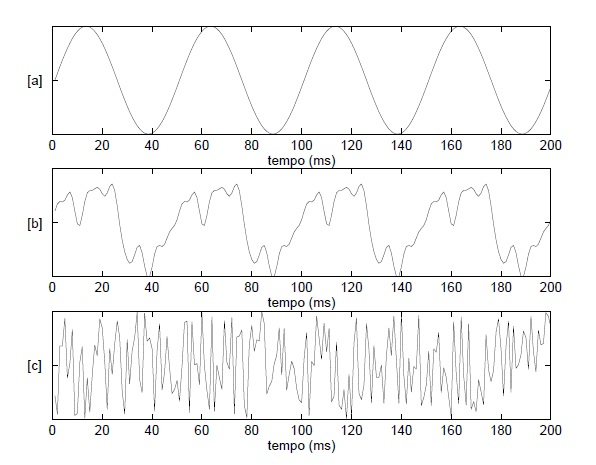
\includegraphics[height=90mm]{img/forma_onda}}
\caption{Andamento nel tempo di tre segnali, rispettivamente: [a] sinusoidale, [b] periodico (somma di 16 sinusoidi), [c] aperiodico.}
\label{fig:forma_onda}
\end{figure}


		\subsubsection{Inviluppo}
		\label{cap2sec1_1_1}
			L'andamento dell'ampiezza di un suono dal momento in cui viene generato fino a quando si estingue viene chiamato inviluppo, in particolare ogni suono ha un inizio e una fine.\\
Prendiamo come esempio la generazione di un suono da una corda di violino eccitata con l'archetto. In condizioni di riposo la corda ha ovviamente vibrazione nulla, e quindi non produce alcun suono. Quando il violinista inizia a sfregare l'archetto sulla corda, questa inizia a vibrare abbandonando la situazione di riposo. Esiste un periodo di tempo nel quale le oscillazioni della corda, da nulle, si fanno sempre più ampie. Questa viene definita fase di attacco e solitamente indicata con il corrispondente termine inglese {\itshape attack}. Questa fase dura solitamente pochi centesimi di secondo, in relazione al tipo di strumento musicale. La fase successiva è definita con il termine inglese {\itshape decay}: corrisponde ad un rapido assestarsi dell'ampiezza ad un valore stabile dopo una sovraelongazione a cui è stata portata dalla fase di attacco. A questo punto, esaurito il transitorio di attacco, si è realizzato un accoppiamento tra lo sfregamento dell'archetto e le oscillazioni della corda. Questo corrisponde alla fase di {\itshape sustain}, che può durare anche parecchi secondi, nella quale il suono viene appunto sostenuto dal musicista, che continua a fornire l'energia necessaria per mantenere le vibrazioni. L'ultima fase, che ha inizio nel momento in cui il musicista smette di mantenere eccitato il sistema di vibrazione, viene denominata {\itshape release} (ovvero rilascio) e corrisponde al tempo in cui il corpo vibrante (nel nostro esempio la corda di violino) smorza l’entità delle vibrazioni, fino a portarsi nuovamente nello stato di quiete.

\begin{figure}[htbp]
\centerline{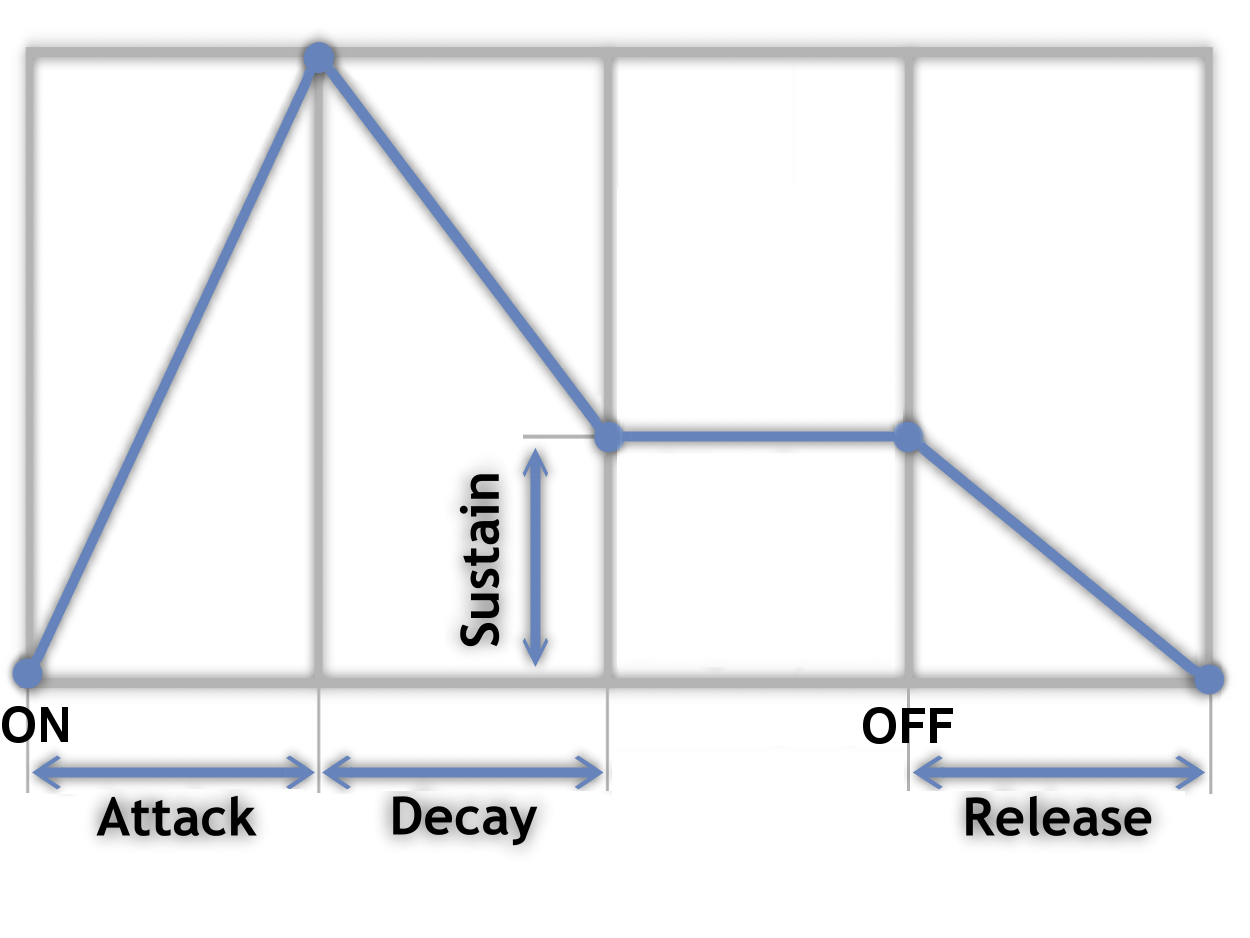
\includegraphics[height=60mm]{img/adsr}}
\caption{Inviluppo - ADSR}
\label{fig:adsr}
\end{figure}
		
		\subsubsection{Altezza}
		\label{cap2sec1_1_2}
			Il primo parametro percettivo che andremo a descrivere è l'altezza di un suono, ovvero la frequenza. La frequenza è una grandezza che indica il numero di oscillazioni compiute in un secondo e  riguarda fenomeni periodici o fenomeni ripetitivi.\\
In campo musicale si è soliti descrivere un suono periodico in termini di frequenza, usualmente indicata con il simbolo $f$ e misurata in Hertz(Hz). Il legame tra periodo $T$ e frequenza $f$ è descritto dalla formula:

$$ f = \frac{1}{T} $$

Come vedremo di seguito un suono periodico di frequenza $f$ può essere scomposto in forme d'onda elementari con frequenze rispettivamente $f$, 2$f$, 3$f$, 4$f$,\dots. La sinusoide di frequenza $f$, pari alla frequenza del suono periodico di partenza è detta {\itshape fondamentale}, mentre le sinusoidi di frequenza multipla intera di $f$ vengono dette parziali o {\itshape armoniche}.

Le caratteristiche frequenziali inducono una differenziazione dei suoni in suoni puri e complessi.\\
Un suono puro (detto anche tono) è costituito da una sola frequenza ed è quindi descritto da un'onda sinusoidale semplice;\\
Un suono complesso consiste invece di più frequenze sommate in un'onda dall'andamento articolato; in un singolo periodo possono essere comprese più alternanze di compressioni e rarefazioni intermedie. In generale in natura i suoni sono di tipo complesso, e lo specifico andamento deriva dal metodo di produzione del suono da parte della sorgente.

		\subsubsection{Intensità}
		\label{cap2sec1_1_3}
		Si è detto che l'equivalente fisico del suono è la variazione di pressione nell'aria. L'entità delle variazioni di pressione è legata alla percezione di volume sonoro ({\itshape loudness}): maggiore è la variazione di pressione, maggiore sarà il volume sonoro percepito.\\
I valori di pressione, potenza e intensità acustica dei suoni si distribuiscono in un intervallo di valori molto esteso. Per questa ragione queste grandezze sono comunemente espresse in scala logaritmica.
Va inoltre osservato che la scala logaritmica ha un andamento più vicino a quello delle scale percettive del nostro apparato uditivo.
L'orecchio umano è in grado di percepire intensità acustiche che variano in un intervallo molto grande (12 ordini di grandezza): si definisce soglia di udibilità il valore $I = 10^{-12} W/m^2$ al di sotto del quale non è più possibile percepire alcun rumore, mentre si chiama soglia del dolore il valore $I = 1 W/m^2$ al di sopra del quale si inizia a provare dolore fisico.\\
Viene definito come livello di pressione acustica ($PL$), misurata in decibel (dB) il logaritmo del rapporto tra la pressione misurata e una pressione di riferimento. In formule:
$$ PL = 20 \cdot \log_{10} \frac{p}{p_{ref}}   $$
dove $p$ è un valore di pressione e $p_{ref}$ è il valore di pressione di riferimento.\\
Può risultare comunque conveniente utilizzare come riferimento la minima pressione efficace udibile $p_0 = 0,00002 Pa$; in questo caso si parla di Sound Pressure Level (SPL).

\clearpage

\begin{table}[h]
\begin{center}
\begin{tabular}{|c|c|r|}
\hline
{\bfseries Indicazione} & Sorgente sonora & Intensità (dB) \\
\hline
& Silenzio & 0 \\

& Spillo che cade & 10\\

& Sussurro a 1 m & 20\\

& Sala vuota & 30\\

$ppp$ & Libreria & 40\\

$pp$ & Interno auto silenziosa & 50\\

$p$ & Conversazione pacata & 60\\

$mp$ & Traffico & 70\\

$mf$ & Fabbrica & 80\\

$f$ & Metropolitana & 90\\

$ff$ & Discoteca & 100\\

$fff$ & Concerto rock & 110\\

& Jet in partenza a 500 m & 120\\
\hline
\end{tabular}
\end{center}
\caption{Livello di intensità associato alle indicazioni di partitura (prima colonna) e prodotto da alcune sorgenti sonore (seconda colonna). (I valori riportati vanno presi come puramente indicativi)}
\label{tab:decibel}
\end{table}
	
		\subsubsection{Timbro}
		\label{cap2sec1_1_4}	
		Il timbro è quella particolare qualità del suono che permette di distinguere due suoni, rappresenta dunque, quell'attributo della sensazione uditiva che consente all'ascoltatore di identificare la fonte sonora, rendendola distinguibile da ogni altra.\\
Una nota suonata da un pianoforte avrà un timbro differente rispetto alla stessa nota prodotta da un violino o da un flauto.
Il timbro è determinato dalle caratteristiche fisiche dello strumento, quali il mezzo utilizzato per produrre il suono (corde, pelle, ancia, \dots), dipendente prevalentemente dalle {\itshape zone formanti}, o semplicemente dette {\itshape formanti}.\\
Per formante s'intende una frequenza di risonanza attorno alla quale un suono spettralmente ricco ha un picco di ampiezza, sono zone in frequenza dove vi è una notevole concentrazione di energia. Non devono essere confuse con le costituenti armoniche del suono.\\

Nella voce umana le formanti sono dovute alle risonanze del tratto vocale, ma esse possono essere individuate anche nell'emissione di strumenti acustici, ad esempio, nei cordofoni, le formanti sono il risultato delle risonanze della tavola armonica. Il tratto vocale e la tavola armonica sono esempi di filtri che, applicati alla vibrazioni di corde, creano formanti atti al riconoscimento del timbro di un determinato strumento.

\begin{figure}[htbp]
\centerline{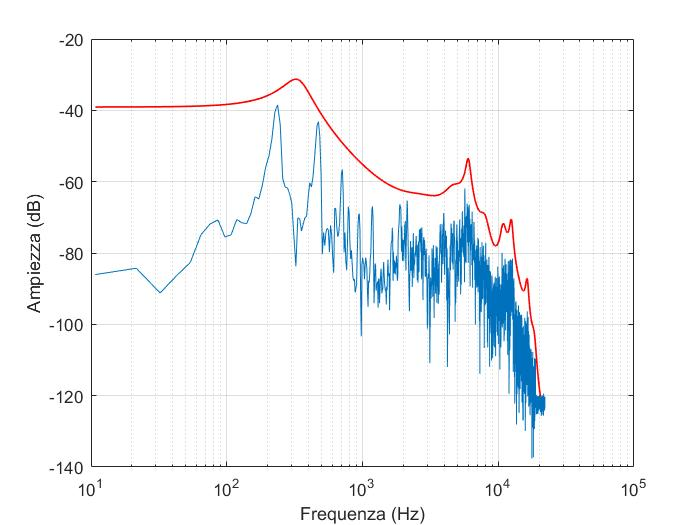
\includegraphics[height=100mm]{img/formant}}
\caption{Esempio di formanti (linea continua rossa)}
\label{fig:formant}
\end{figure}
	
%	\section{Analisi segnali nel dominio della frequenza}
	\label{cap2sec3}
	
% Verranno ora fornite informazioni di base sull'analisi in frequenza dei segnali.
		
	
		\subsection{Segnali Periodici}
		\label{cap2sec3_1}
		
		Una delle classi di segnali cui si farà riferimento all'interno di questo elaborato è quella dei segnali che si ripetono periodicamente nel tempo, detti segnali periodici. 
Più precisamente diremo che un segnale $f(t)$ è periodico al periodo $T$ se si verifica che $$ f(t) = f(t+kT), \qquad \forall t \in \Re $$ 
Il minimo valore del periodo $T > 0$ che soddisfa la definizione di periodicità è chiamato periodo fondamentale ed è denotato da T0. L'inverso di questo valore rappresenta la frequenza fondamentale del segnale.
		
		\subsection{Serie di Fourier}
		\label{cap2sec3_2}
		
		I segnali periodici possono essere rappresentati come combinazione lineare di funzioni sinusoidali complesse mediante l'utilizzo di concetti matematici che prendono il nome di serie e trasformate di Fourier\footnote{La trasformata di Fourier è una generalizzazione ai segnali non periodici}.
		
$$ f(t) = \sum_{n = -\infty}^{\infty} c_ne^{inw_0t} \qquad \mbox{con} \qquad c_n = \frac{1}{T}\int_{-\frac{T}{2}}^\frac{T}{2}f(t)e^{-inw_0t}dt$$

Queste due equazioni matematiche prendono rispettivamente il nome di equazione di sintesi ed equazione di analisi della serie di Fourier. La prima consente di sintetizzare il segnale $ f(t) $ sovrapponendo le singole funzioni complesse, la seconda, invece, consente di decomporlo calcolandone i coefficienti complessi.
Mediante l'identità di Eulero è possibile riscrivere queste equazioni utilizzando funzioni trigonometriche.

$$ \mbox{cos}(\theta) + i\mbox{sen}(\theta) = e^{i\theta} $$
$$ f(t) = \sum_{n=-\infty}^\infty c_n e^{inw_0t} = \frac{a_0}{2} + 
\sum_{n=1}^\infty [a_n\mbox{cos}(nw_0t)+ b_n\mbox{sin}(nw_0t)]$$

Dall'equazione precedente si nota che tutti i segnali periodici possono essere rappresentati come sovrapposizioni di funzioni trigonometriche con frequenza multipla di una frequenza data.
				
		\subsection{Trasformata di Fourier}
		\label{cap2sec3_3}
		
		La trasformata di Fourier consente un'estensione della serie di Fourier e permette la rappresentazione in frequenza di funzioni che, non essendo periodiche, non ammettono una trasformazione in serie di Fourier.\\
Ammettiamo un qualunque segnale come periodico di periodo $T$ con $T\rightarrow\infty$ un segnale $f(t)$ non periodico, chiamiamo $f_T(t)$ la funzione periodica di periodo $T$ che coincide con $f(t)$ nell'intervallo $[-\frac{T}{2},\frac{T}{2}]$; possiamo scrivere:

$$ f(t) = \lim_{T\rightarrow\infty} f_T(t) $$

Essendo $f_T(t)$ una funzione periodica, può essere sviluppata in serie di Fourier:

$$ f(t) = \sum_{n = -\infty}^{\infty} c_ne^{inw_0t} \qquad \mbox{con} \qquad c_n = \frac{1}{T}\int_{-\frac{T}{2}}^\frac{T}{2}f(t)e^{-inw_0t}dt$$

Sapendo che $w_0 = 2\pi v$, chiamiamo $v_n = nv$ la frequenza dell'ennesima armonica e $\Delta v = v_{n+1}-v = \frac{1}{T}$ la distanza tra una frequenza e la successiva; ponendo $F(v) = c_nT$ possiamo scrivere:

$$ f_T(t) = \sum_{n = -\infty}^\infty F(v_n)e^{i2\pi v_nt}\Delta v \qquad 
 \qquad F(v_n) = \int_{-\frac{T}{2}}^\frac{T}{2} f_T(t)e^{-i2\pi v_nt} $$

Per $ T\rightarrow\infty$ e $\Delta v \rightarrow 0$, la serie precedente si riduce ad un integrale:

$$	f(t) = \int_{-\infty}^\infty F(v)e^{i2\pi vt}dv \qquad F(v) = \int_{-\infty}^\infty f(t)e^{-i2\pi vt}dt
$$

$F(v)$ viene chiamata formula di analisi o {\itshape Trasformata di Fourier} e ne rappresenta il contenuto in frequenza del segnale $f(t)$, ovvero il suo contenuto spettrale.\\
$f(t)$ viene chiamata, invece, formula di ricostruzione o {\itshape Anti-trasformata di Fourier}, e permette la ricostruzione di $f(t)$ a partire dal suo contenuto in frequenza: $f(t)$ viene scomposta in un numero infinito di sinusoidi continue complesse.	
\\

\begin{figure}[htbp]
\centerline{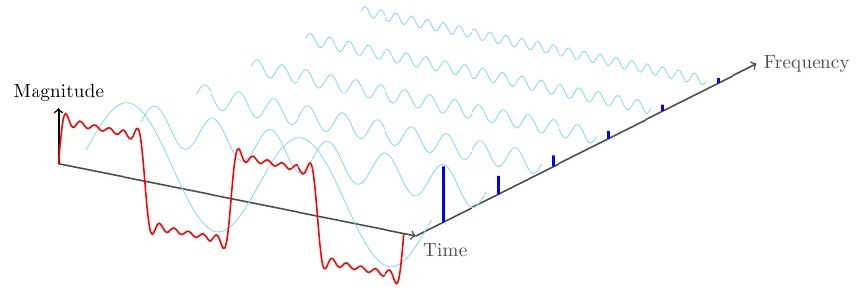
\includegraphics[height=60mm]{img/fourier_transform}}
\caption{Dominio del tempo - frequenza}
\label{fig:fourier_transform}
\end{figure}

La trasformata e l'anti-trasformata di Fourier operano su segnali continui nel tempo e delle frequenza. \\
Per poterle operare in un calcolatore digitale è necessario adottare una discretizzazione dei segnali, introducendo una versione discreta della trasformata, la trasformata discreta di Fourier (DFT).

		\subsubsection{DFT}
		\label{cap2sec3_4}
		Consideriamo il segnale $f_s(t)$ ottenuto campionando $f(t)$ ai tempi $n\tau(-\infty < n < \infty)$, con $\tau$ corrispondente il passo di campionamento, mediante una funzione impulsiva $\delta(t)$. L'informazione contenuta nel segnale $f(t)$ viene approssimata con quella contenuta nel vettore discreto $x$ formato da $N$ campioni del segnale campionato con passo $\tau$.

$$ x(n) = f(n\tau) \qquad \mbox{con} n=0,\dots,N-1 $$

L'informazione in frequenza di questa funzione viene calcolata mediante la trasformata di Fourier dell'espressione precedente; essendo il segnale considerato un segnale campionato e quindi discreto, questa operazione prende il nome di {\itshape Trasformata di Fourier a tempo Discreto} $(DTFT)$; sapendo che $F(\delta(t-n\tau)) = e^{-i2\pi vn\tau} $ otteniamo:

$$ F_s(v) = \sum_{n = -\infty}^\infty x(n)e^{-2\pi vn\tau} $$

La funzione $F_s(v)$ rappresenta lo spettro continuo del segnale $x(n)$, è necessario campionare anche il dominio della frequenza con intervalli equidistanti di ampiezza pari a $F_0 = \frac{f_s}{N}$ con $f_s = \frac{1}{\tau} = \mbox{\itshape frequenza di campionamento}$ dove $F_0$ corrisponde alla risoluzione frequenziale della $DFT$.

Sapendo che :
$$ X(k) = F_s(kF_0) \qquad \mbox{con} \qquad k = 0,\dots,N-1 $$

otteniamo:
$$ X(k) = \sum_{n=0}^{N-1} x(n)e^{-i2\pi kF0n\tau} = 
		\sum_{n=0}^{N-1} x(n)e^{-i2\pi k\frac{1}{N\tau}n\tau} =
			\sum_{n=0}^{N-1} x(n)e^{-ik\frac{2\pi}{N}n}	$$

Quindi:

$$ X(k) = \sum_{n = 0}^{N-1} x(n)e^{-ik\frac{2\pi}{N}n} \qquad \mbox{\&} \qquad
	x(n) = \frac{1}{N}\sum_{n=0}^{N-1} X(k)e^{ik\frac{2\pi}{N}n} $$

Queste due espressioni prendono il nome di trasformata e anti-trasformata discrete di Fourier.

Essendo il risultato della DFT una successione di numeri complessi, la trasformata permette di ottenere informazioni riguardo l'ampiezza e la fase delle diverse componenti sinusoidali del segnale in ingresso.\\
Queste due informazioni possono essere ottenute esprimendo i valori complessi in forma polare, ottenendo così l'ampiezza $A_k$ e la fase $\phi_k$ delle sinusoidi rispettivamente dal modulo e argomento di $X_k$:

$$ A_k = |X_k| = \sqrt{{\mbox{Re}(X_k)}^2 + \mbox{Im}(X_k)^2} \qquad \mbox{\&} \qquad
	\varphi_k = \mbox{arg}(X_k) = \mbox{atan}(\mbox{Im}(X_k),\mbox{Re}(X_k)) $$
		
		\subsubsection{STFT}
		\label{cap2sec3_5}
		La trasformata di Fourier permette di ottenere informazioni delle componenti armoniche nel segnale, ma non permette di avere una valutazione temporale di quando tali frequenze siano effettivamente presenti, occorre inserire una dipendenza dal tempo nella trasformazione.
Dividendo il segnale in segmenti di lunghezza fissa, si riescono ad avere informazioni circa la variazione in frequenza nel tempo effettuando la trasformata di Fourier per ogni segmento finestrato:

$$ STFT_x(\tau,v) = \int_{-\infty}^{+\infty} x(t)g(t-\tau)e^{i2\pi vt}dt $$

L'espressione precedente prende il nome di trasformata di Fourier a breve termine o Short Time Fourier Transform (STFT).

Il segnale viene modificato dal comportamento della finestra presa in esame\footnote{Esistono molteplici tipologie di finestre : Hamming, Hann, Blackman, Gauss, Blackman-Harris etc\dots}, di conseguenza la STFT fornisce lo spettro del segnale alterato dalla presenza della finestra.\\
In questo senso una finestra che nel dominio del tempo provoca al segnale rapide transizioni, nel dominio della frequenza causa una forte dispersione {\itshape leakage} della potenza su tutto lo spettro come ad esempio la finestra rettangolare.
\\

Le caratteristiche fondamentali di una finestra sono: il fattore di dispersione, la larghezza del Mainlobe (lobo principale) e l'attenuazzione in dB del Sidelobes (lobi laterali).\\
Una finestra ideale dovrebbe avere un fattore di dispersione uguale a zero, una larghezza del Mainlobe molto bassa e un'attenuazione in dB del Sidelobe molto alta. Di seguito si illustrano due esempi di due finestre: la finestra rettangolare e la finestra di Hamming.
\clearpage
Nella figura \ref{fig:rect_fun} si può notare una bassissima attenuazione del Sidelobe: intorno ai $-13$ dB, un fattore di dispersione del $9\%$

\begin{figure}[htbp]
\centerline{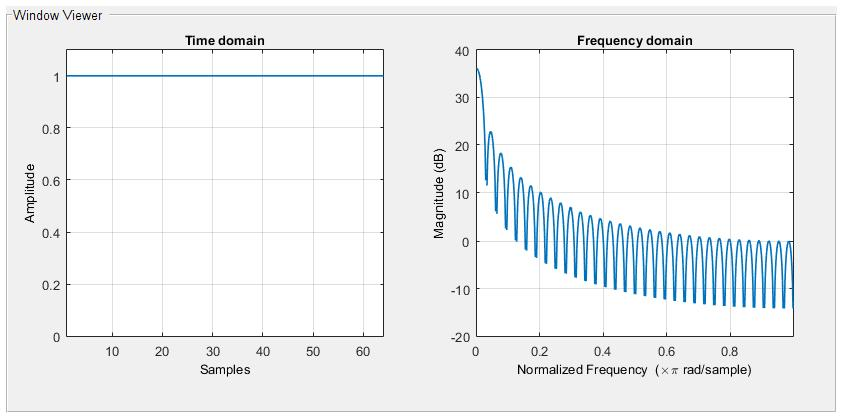
\includegraphics[height=60mm]{img/rect_fun}}
\caption{Finestra rettangolare}
\label{fig:rect_fun}
\end{figure}

Nella figura \ref{fig:hamming_fun} si può notare, invece che l'attenuazione dei sidelobes è molto più alta rispetto alla finestra rettangolare: intorno a $-42$ dB, questo comporterebbe una miglior lettura della STFT e un fattore di dispersione del $0.03\%$\footnote{I dati esposti sono stati elaborati tramite il tool in MATLAB "wvtool"}

\begin{figure}[htbp]
\centerline{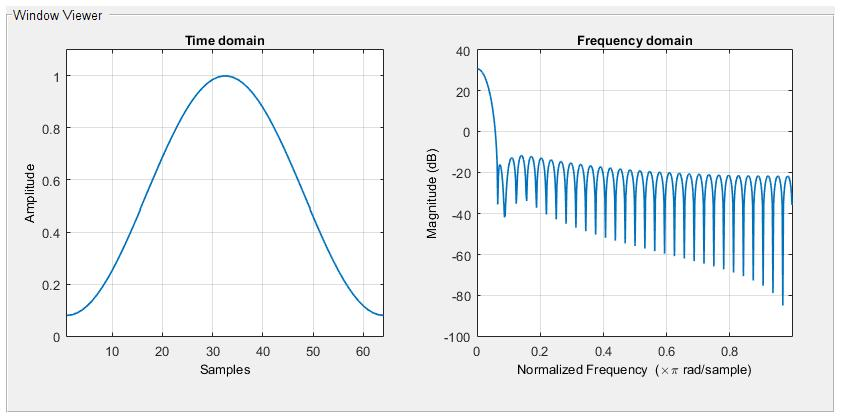
\includegraphics[height=60mm]{img/hamming_fun}}
\caption{Finestra di Hamming}
\label{fig:hamming_fun}
\end{figure}

\clearpage

La finestra utilizzata per la maggior parte all'interno dell'elaborato è la finestra di Hamming perchè garantisce un ottimo compromesso tra larghezza del mainlobe (una buona precisione frequenziale) e una notevole attenuazione dei sidelobes (miglior definizione dello spettrogramma).
\\\\

Di seguito si illustra un esempio di sonogramma di un fraseggio di chitarra.
\begin{figure}[htbp]
\centerline{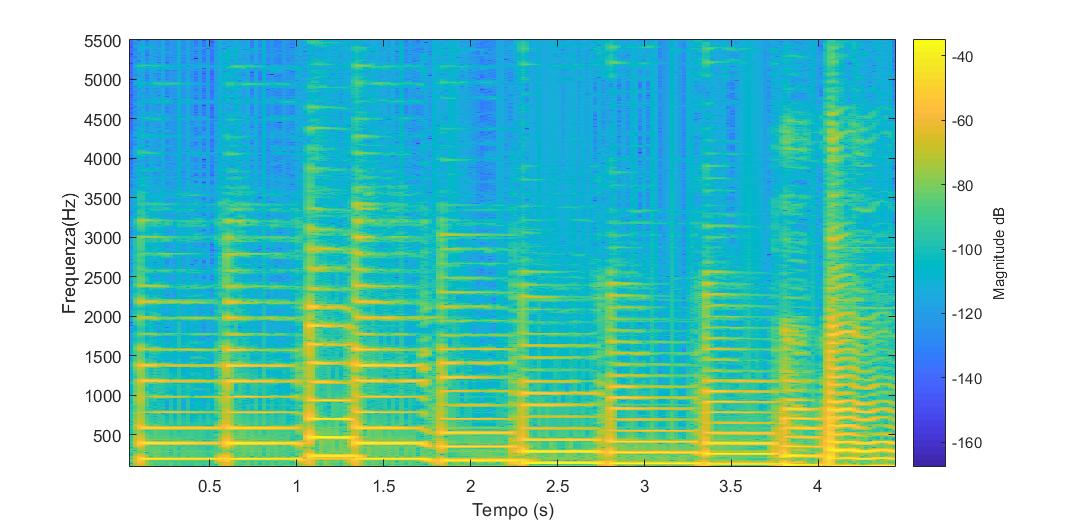
\includegraphics[height=90mm]{img/sonogram}}
\caption{Sonogramma}
\label{fig:sonogram}
\end{figure}

\chapter{Modello di Analisi}
\label{cap3}
	Come già accennato nell'introduzione, questo lavoro effettua analisi di coppie di segnali simili, ne estrae {\itshape features} caratteristiche e ne calcola le differenze.
	
	In questo capitolo si illustrerà il modello di analisi utilizzato e le relative implementazioni utilizzando come segnali di test segnali ideali per convalidare il modello, per poi analizzare suoni reali come chitarre e voci.\\
Verranno generati toni puri e chirp per convalidare il modello {\itshape Analisi armonica - Harmonic tracking} (\ref{cap3sec2}); verranno utilizzati impulsi per validare la precisione del modello {\itshape Analisi attacco delle note - Onset Detection} (\ref{cap3sec4}); Per quanto riguarda la sezione {\itshape Analisi della dinamica (\ref{cap3sec1})} e  {\itshape Analisi timbrica - Rilevamento delle formanti} (\ref{cap3sec3}) verranno utilizzati, invece, segnali complessi come chitarre e voci.\\

	\section{Analisi della dinamica}
	\label{cap3sec1}
	In questa sezione verranno estratte {\itshape features} che caratterizzano la dinamica di una segnale audio, ovvero verrà calcolato: il {\itshape valore efficace} del segnale (RMS), il {\itshape valore massimo di ampiezza} (valore di picco) e il valore di {\itshape crest factor} (misura del range dinamico).

Prendiamo in considerazione un piccolo riff di chitarra elettrica, dopo averlo diviso in segmenti di lunghezza di $1024$ campioni ($23.2$ ms = lunghezza finestra di analisi) utilizzando un overlapping del $75\%$, calcoliamo il valore efficace mediante la formula del {\itshape valore quadratico medio}:
\clearpage
$$ x_{rms} = \sqrt{\frac{1}{n}\sum_{i=1}^n x_i^2}$$
dove $n$ è la lunghezza del segmento e $x_i$ è il valore di ampiezza del segnale.
In questo modo calcoliamo ogni $23.2$ ms il valore efficace del suono, ovvero il valore efficace della variazione della pressione sonora.

Allo stesso modo calcoliamo il valore massimo di ampiezza e il crest factor\footnote{Valore normalizzato tra 0 e 1} rispettivamente:

$$ x_{picco} = \mbox{max}(|x|) \qquad \mbox{\&} \qquad x_{crest} = \frac{x_{picco}}{x_{rms}}$$

Infine, dato che i valori del segnale sono rappresentati tra $-1$ e $1$, dalla formula presente nella sottosezione \ref{cap2sec1_1_3}, possiamo convertirli in decibel mediante la formula:

$$ dB_{fs}(A) = 20 \cdot \log{10}(A) $$

I risultati ottenuti sono rappresentati nella Fig. \ref{fig:wave_rms_picco}

\begin{figure}[htbp]
\centerline{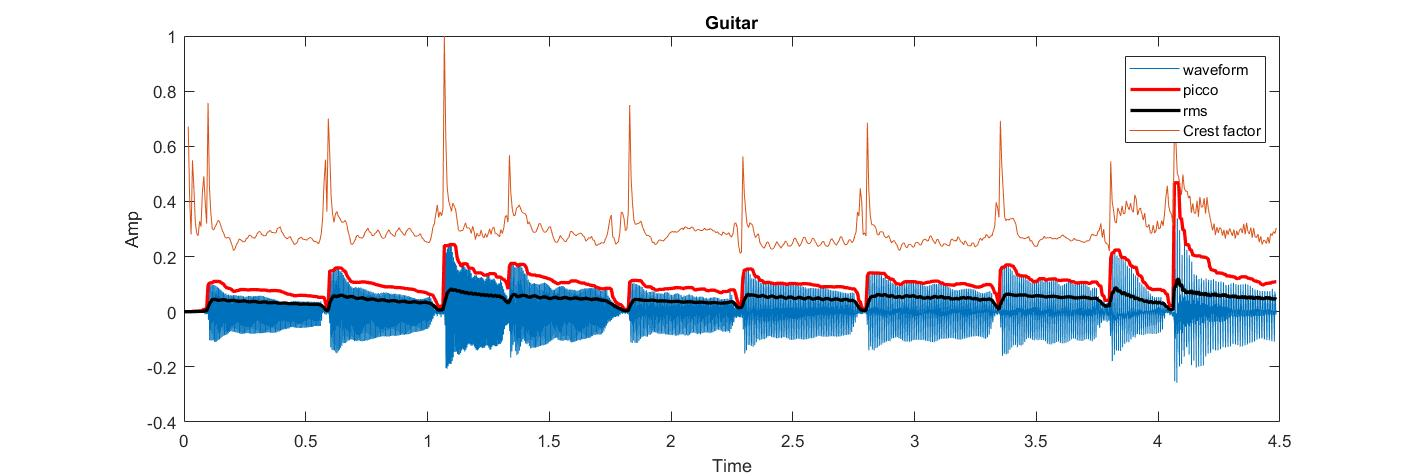
\includegraphics[height=60mm]{img/wave_rms_piccoa}}
\caption{Esempio segnale audio - riff di chitarra}
\label{fig:wave_rms_picco}
\end{figure}

\clearpage

	\section{Analisi armonica - Harmonic tracking}
	\label{cap3sec2}
		Utilizzando la tecnica della doppia incisione, le tracce create sono molto simili tra di loro, ma non saranno mai identiche. Questo è dovuto alle microvariazioni introdotte dall'esecutore durante la sua performance. Prendiamo in considerazione, ora, le variazioni in frequenza, per le variazioni nel tempo si faccia riferimento alla sezione (\ref{cap3sec4}).\\
Prendiamo come esempio un'incisione di chitarra, qualsiasi essa sia, le microvariazioni in frequenza sono dovute da molteplici fattori quali: umidità dell'aria, temperatura, qualità delle componenti dello strumento, pressione del dito sulla corda e la posizione del dito all'interno del tasto ({\itshape fret}).\\
In questa sezione si andrà ad esporre le tecniche utilizzate per il tracciamento delle armoniche illustrando i relativi risultati tramite segnali di test ideali (toni puri, chirp).

		\subsection{Interpolazione parabolica}
		\label{cap3sec2_1}
		Il primo metodo proposto prende in considerazione un modello matematico, il calcolo del vertice di una parabola passante per tre punti.\\
Nel capitolo precedente (sezione \ref{cap2sec3_5}) si è vista l'importanza della tipologia della finestra di analisi per avere una miglior precisione sui picchi nel dominio della frequenza, per aumentare tale risoluzione possiamo aumentare la dimensione della finestra di analisi, questo comporterebbe una finestra molto grande, con lo svantaggio di avere un calcolo computazionale molto elevato.
Nella figura \ref{fig:peak} si illustra il rilevamento del picco in frequenza di una sinusoide di frequenza 880 Hz, si noti che entrambi i picchi non coincidono con il valore perfetto dell'oscillazione .\\

\begin{figure}[htbp]  \centering 
	\begin{minipage}[c]{.40\textwidth} 
		\centering
		%\setlength{\captionmargin}{0pt}% 
		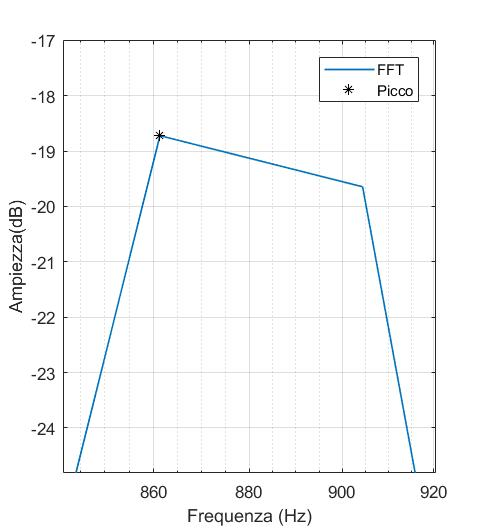
\includegraphics[width= 1.2 \textwidth]{img/1024peak} 
		%\caption{Immagine piccola} 
	\end{minipage}% 
	\hspace{10mm}% 
	\begin{minipage}[c]{.40\textwidth} 
		\centering
		%\setlength{\captionmargin}{0pt}% 
		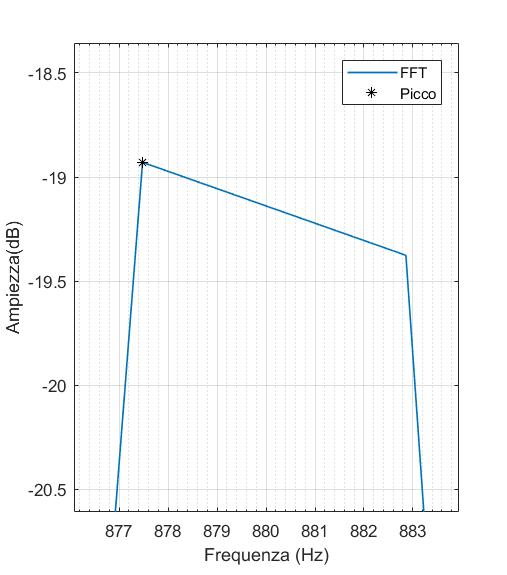
\includegraphics[width= 1.2 \textwidth]{img/8192peak} 
		%\caption{Immagine grande} 
	\end{minipage} 
	\caption{Picco in frequenza di una sinusoide di 880 Hz calcolando la FFT con finestre di 1024 campioni (a sinistra) e 8182 campioni (a destra).}
	\label{fig:peak}
\end{figure} 

La soluzione a questo problema è effettuare un'interpolazione parabolica\cite{parshl}. Una parabola è una funzione con la forma molto simile alla forma del lobo nello spettro della finestra di analisi, in scala logaritmica.

In un insieme di coordinate centrato a ($k_\beta,0$), dove $k_\beta$ è numero del bin a cui fa riferimento il picco massimo di magnitudine $mX(k_\beta)$ (designato come asterisco in figura), definiamo la funzione parabola tramite la forma

$$ x(n) = a(n - p)^2 + b $$
tale che $x(-1) = \alpha$, $x(0) = \beta$, $x(1) = \gamma$, dove $\alpha$, $\beta$ e $\gamma$ corrispondono ai valori dei tre {\itshape bin} più alti:

\begin{eqnarray*}
	\alpha & = & mX[k_\beta - 1] \\
	\beta & = & mX[k_\beta] \\
	\gamma & = & mX[k_\beta + 1]
\end{eqnarray*}

\begin{figure}[htbp]
\centerline{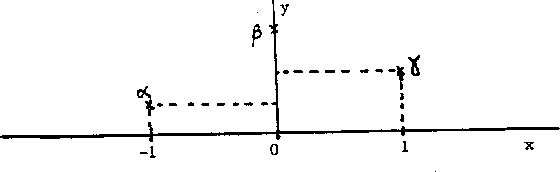
\includegraphics[height=40mm]{img/parab}}
\caption{Coordinate dell'interpolazione parabolica}
\label{fig:parab}
\end{figure}
Dall'equazione generale della parabola calcoliamo la locazione {\itshape p} corrispondente al vertice della parabola ricostruita, ottenendo così lo scostamento dal bin del picco rilevato alla posizione ($k_\beta, 0$):

$$ p = \frac{1}{2} \frac{\alpha - \gamma}{\alpha - 2\beta + \gamma} $$
Il valore del bin corrispondente alla posizione veritiera si ottiene sommando lo scostamento appena rilevato alla posizione $k_\beta$

$$ \mbox{\^{k}} = k_\beta + p $$
ottenendo il valore in Hz con la formula 

$$ \frac{f_s\cdot \mbox{\^{k}}}{N}$$
dove $f_s$ corrisponde alla {\itshape frequenza di campionamento}.\\
Infine il valore di ampiezza corrispondente al vertice calcolato:

$$ x(p) = \beta - \frac{1}{4}(\alpha - \gamma)p  $$

Di seguito si illustra il risultato dell'interpolazione sulla sinusoide di test. La figura di sinistra rappresenta un picco al valore di 878.1297 Hz, mentre la figura di destra a 879.8692 Hz.

\begin{figure}[htbp]  \centering 
	\begin{minipage}[c]{.40\textwidth} 
		\centering
		%\setlength{\captionmargin}{0pt}% 
		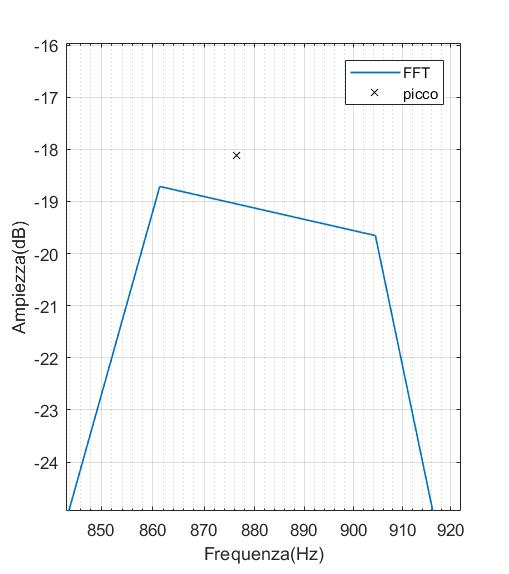
\includegraphics[width= 1.14 \textwidth]{img/1024peak_parab} 
		%\caption{Immagine piccola} 
	\end{minipage}% 
	\hspace{10mm}% 
	\begin{minipage}[c]{.40\textwidth} 
		\centering
		%\setlength{\captionmargin}{0pt}% 
		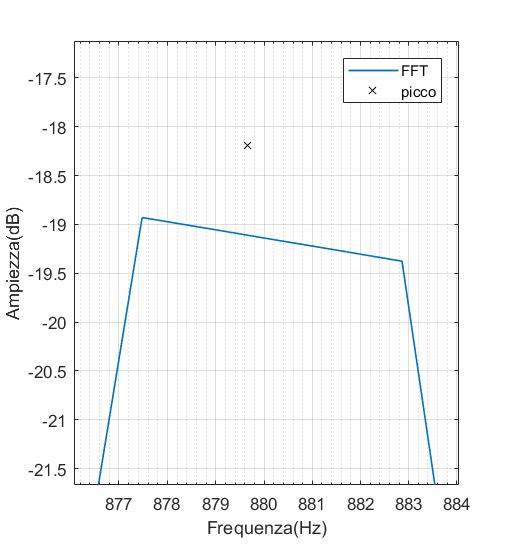
\includegraphics[width= 1.2 \textwidth]{img/8192peak_parab} 
		%\caption{Immagine grande} 
	\end{minipage} 
	\caption{Interpolazione parabolica effettuata su una sinusoide di 880 Hz calcolando la FFT con finestre di 1024 campioni (a sinistra) e 8182 campioni (a destra).}
	\label{fig:peak_parab}
\end{figure} 

		\subsection{Differenza di fase}
		\label{cap3sec2_2}
			L'interpolazione parabolica permette di estrarre valori vicini al valore veritiero, ma nel nostro caso non è abbastanza preciso. Per avere una precisione maggiore si descrive un metodo che prende in considerazione la fase del segnale.\\
			
Come si è descritto in precedenza, un segnale può essere scomposto come somma di sinusoidi complesse con valori ben definiti di {\itshape frequenza, fase} e {\itshape magnitudine}, questi valori caratterizzano una sinusoide in un dato istante ({\itshape frame}).\\
La frequenza della sinusoide viene discretizzata in base alla risoluzione spettrale $\frac{f_s}{N}$, dove $f_s$ corrisponde alla frequenza di campionamento e $N$ corrisponde alla lunghezza della finestra di analisi, questo dato corrisponde al valore in frequenza tra un bin e quello successivo. Nel caso in cui la frequenza del segnale coincida esattamente con la frequenza del bin (valore multiplo di $\frac{f_s}{N}$), lo spettro risulterà assente di {\itshape leakage} perchè la finestra non provocherà rapide transizioni dovute al troncamento del segnale. Nel caso in cui la frequenza del segnale non sia multipla di $\frac{f_s}{N}$ il segnale subirà dei ripidi troncamenti alle estremità della finestra. Di seguito si illustra una sinusoide divisa in sette frame.

\begin{figure}[htbp]  \centering 
	\begin{minipage}[c]{.40\textwidth} 
		\centering
		%\setlength{\captionmargin}{0pt}% 
		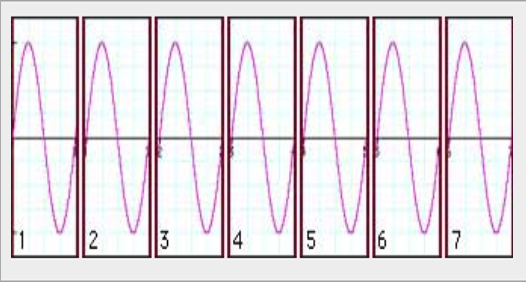
\includegraphics[width= 1.0 \textwidth]{img/inphase} 
		%\caption{Immagine piccola} 
	\end{minipage}% 
	\hspace{10mm}% 
	\begin{minipage}[c]{.40\textwidth} 
		\centering
		%\setlength{\captionmargin}{0pt}% 
		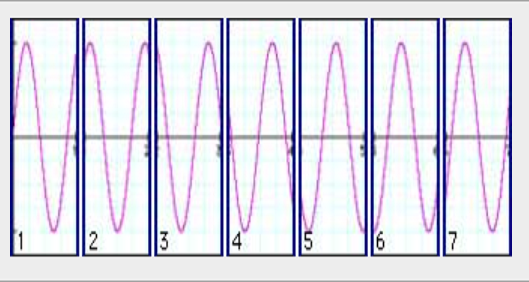
\includegraphics[width= 1.0 \textwidth]{img/nonphase} 
		%\caption{Immagine grande} 
	\end{minipage} 
	\caption{A sinistra una sinusoide con frequenza uguale a quella del {\itshape bin}, a destra una sinusoide con frequenza non corrispondente a quella del {\itshape bin}}
	\label{fig:phase}
\end{figure} 
			
Come si può notare, nella figura di sinistra, ad ogni frame il segnale inizia con lo stesso valore di fase, al contrario invece, il segnale nella figura di destra, che ha una frequenza compresa tra due bin, non inizia ogni frame con la stessa fase, chiaramente siamo in presenza di uno {\itshape scostamento di fase}. Più è alto è lo scostamento, maggiore sarà la deviazione tra il bin di riferimento.
\\
La variazione dello scostamento di fase viene usata per calcolare il valore esatto della frequenza della sinusoide.

Prendendo in considerazione il noto modello di estrazione della frequenza istantanea $f_i[k]$ di Flanagan e Golden \cite{phase1}, si ottiene:

$$ f_i[k] = (k + \kappa[k])\frac{f_s}{N} $$
con:

$$ \kappa[k] = \frac{N}{2\pi L}\mbox{princarg}\left[\phi_l[k] - \phi_{l-1}[k] -
	\frac{2\pi L}{N}k \right[ $$
dove $L$ indica il numero di campioni tra una finestra e quella successiva, comunemente chiamato {\itshape stepsize} oppure {\itshape hopsize} , $k$ corrisponde al bin in frequenza, $\phi_l[k]$ indica il valore della fase al $k$-esimo bin del frame $l$ e $\kappa$ corrisponde alla deviazione in bin della frequenza istantanea dal bin di riferimento. La funzione {\itshape princarg} permette di mappare il valore di fase tra $\pm \pi$.

Di seguito si illustra il risultato ottenuto calcolando la frequenza istantanea sulla sinusoide utilizzata nell'interpolazione parabolica. La figura di sinistra rappresenta un picco al valore di 879,7985 Hz, mentre la figura di destra a 879,9991 Hz.

\begin{figure}[htbp]  \centering 
	\begin{minipage}[c]{.40\textwidth} 
		\centering
		%\setlength{\captionmargin}{0pt}% 
		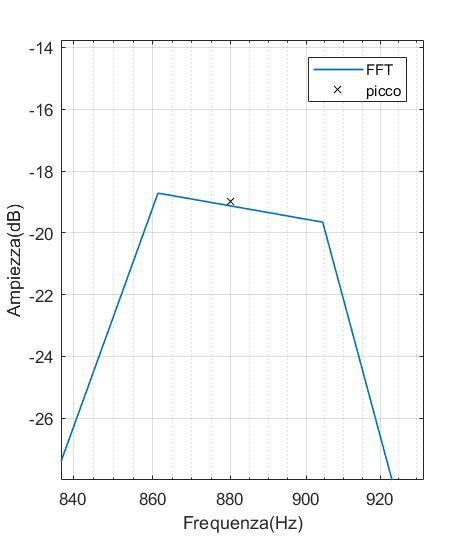
\includegraphics[width= 1.14 \textwidth]{img/1024peak_phase} 
		%\caption{Immagine piccola} 
	\end{minipage}% 
	\hspace{10mm}% 
	\begin{minipage}[c]{.40\textwidth} 
		\centering
		%\setlength{\captionmargin}{0pt}% 
		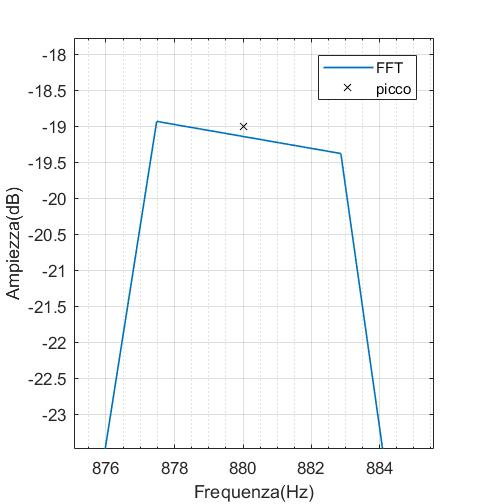
\includegraphics[width= 1.2 \textwidth]{img/8192peak_phase} 
		%\caption{Immagine grande} 
	\end{minipage} 
	\caption{Differenza di fase effettuata su una sinusoide di 880 Hz calcolando la FFT con finestre di 1024 campioni (a sinistra) e 8182 campioni (a destra).}
	\label{fig:peak_phase}
\end{figure} 

\clearpage

	Infine si illustra il risultato sull'intero file audio, rappresentando entrambi i metodi in un'unica figura.

\begin{figure}[htbp]
\centerline{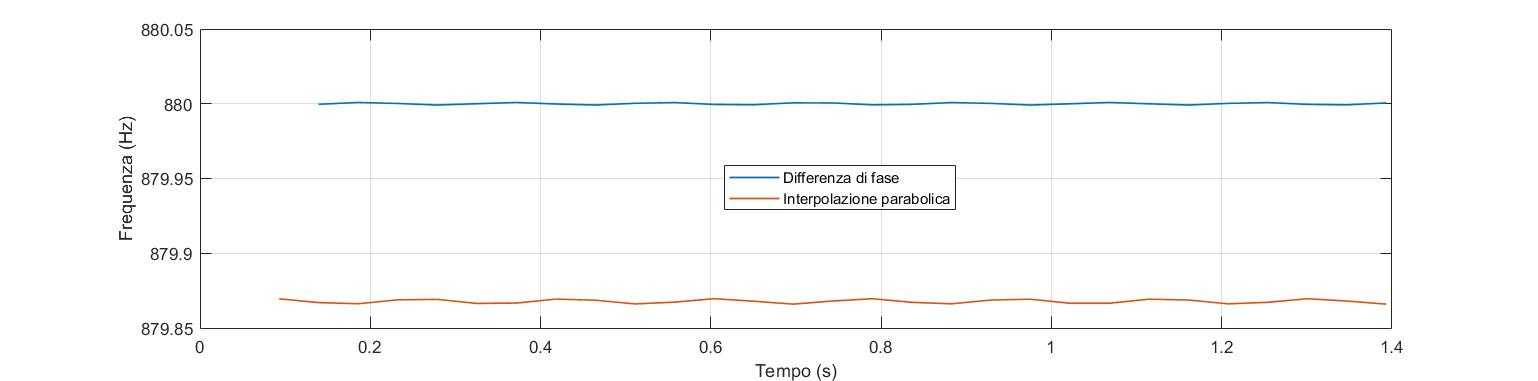
\includegraphics[height=52.5mm]{img/parab_phase}}
\caption{Confronto tra i due metodi}
\label{fig:parab_phase}
\end{figure}

Calcolando la media delle singole tracce, l'implementazione che utilizza la differenza di fase presenta un valore di 880.0000 Hz. Il modello dell'interpolazione parabolica, invece, ha un valore medio di 879.8678 Hz.

	\subsection{Validazione dei modelli}
	\label{cap3sec2_3}
		Ai fini della validazione dei modelli implementati si effettuano ulteriori test su un segnale chirp (da 200 a 500 Hz) e su un segnale complesso quale un riff di chitarra.
		
		\subsubsection{Chirp}
		\label{cap3sec2_3_1}
			Prendiamo in considerazione un segnale ideale che varia la sua frequenza nel tempo, ad esempio un segnale chirp di una durata di tre secondi variando la sua frequenza da 200 Hz a 500 Hz con andamento lineare. Si illustra di seguito i risultati ottenuti da entrambe le implementazioni e il tracciamento del modello più preciso.

In figura \ref{fig:chirp} viene illustrato un frammento di $0.4$ secondi nel passaggio tra i 255 Hz a 295 Hz. Si noti la poca precisione del modello dell'interpolazione parabolica in confronto a quella della differenza di fase. L'andamento lineare in frequenza viene rappresentato correttamente dalla linea blu definendo stabile l'implementazione ottenuta mediante differenza di fase.

\begin{figure}[htbp]
\centerline{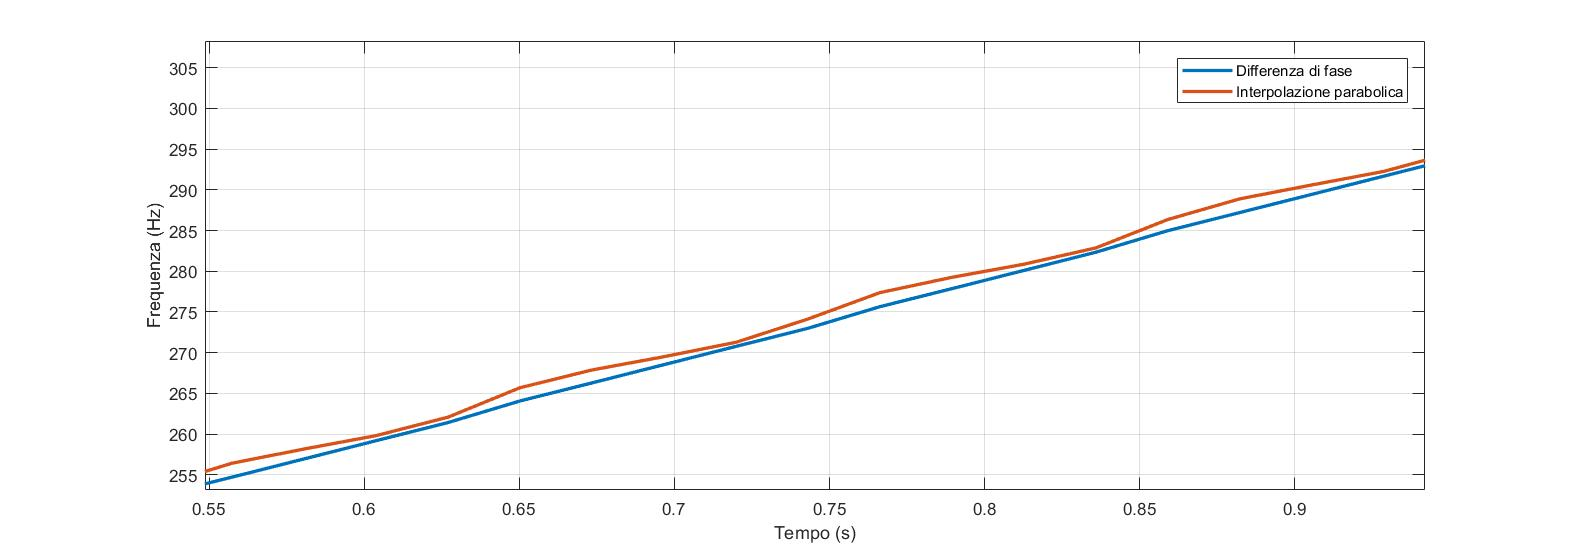
\includegraphics[height=70mm]{img/chirp}}
\caption{Chirp - Differenza di fase e Interpolazione parabolica}
\label{fig:chirp}
\end{figure}

\begin{figure}[htbp]
\centerline{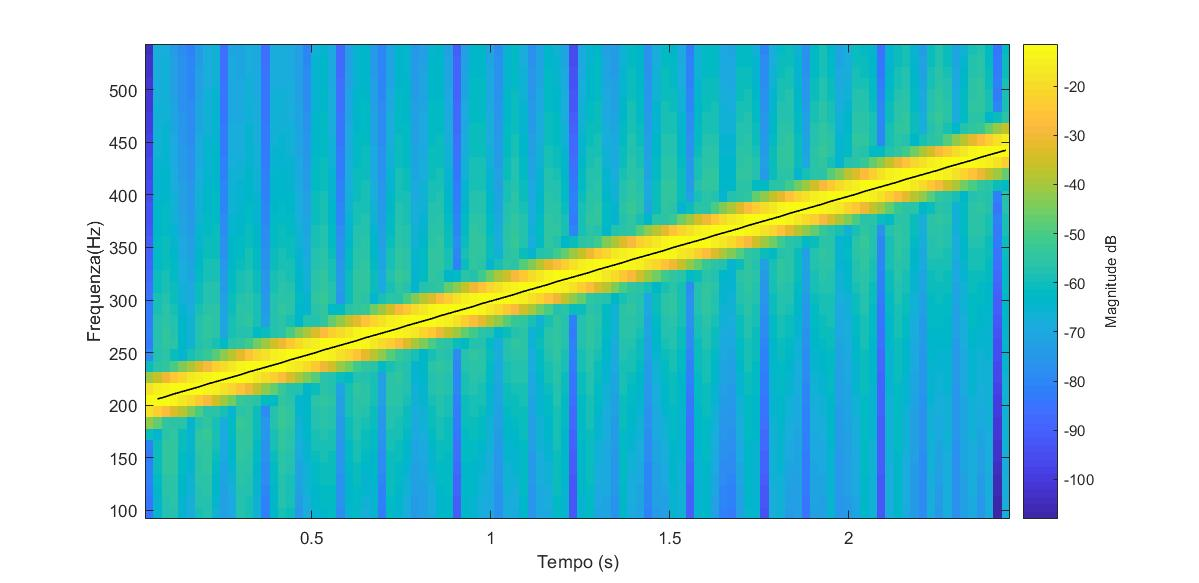
\includegraphics[height=80mm]{img/chirp_sono}}
\caption{Chirp - Sonogramma e relativo tracciamento}
\label{fig:chirp_sono}
\end{figure}

		\subsubsection{Riff di chitarra}
		\label{cap3sec2_3_2}
		Come ultima validazione viene effettuato un test su un segnale complesso dove il suo contenuto spettrale non è più composto da una singola componente, ma di una frequenza fondamentale e dalle sue armoniche.

Prendiamo in esame l'introduzione di chitarra del brano "{\itshape Wither}" del gruppo musicale statunitense Dream Theater. Di seguito si illustra il relativo spettrogramma e il tracciamento delle armoniche (Fig. \ref{fig:wither}).

Il tracciamento viene effettuato seguendo l'andamento dei singoli picchi all'interno del FFT per ogni frame di analisi, analizzando il loro percorso tenendo in considerazione lo scostamento in frequenza tra una nota e quella successiva e scartando errori dovuti da artefatti prodotti dalla finestratura come il rilevamento dei sidelobe fissando una soglia di ampiezza in relazione al valore di SNR prodotto dalla finestra per evitare di rilevare componenti di ampiezza troppo bassa denominati come {\itshape garbage peak}.

\begin{figure}[htbp]
\centerline{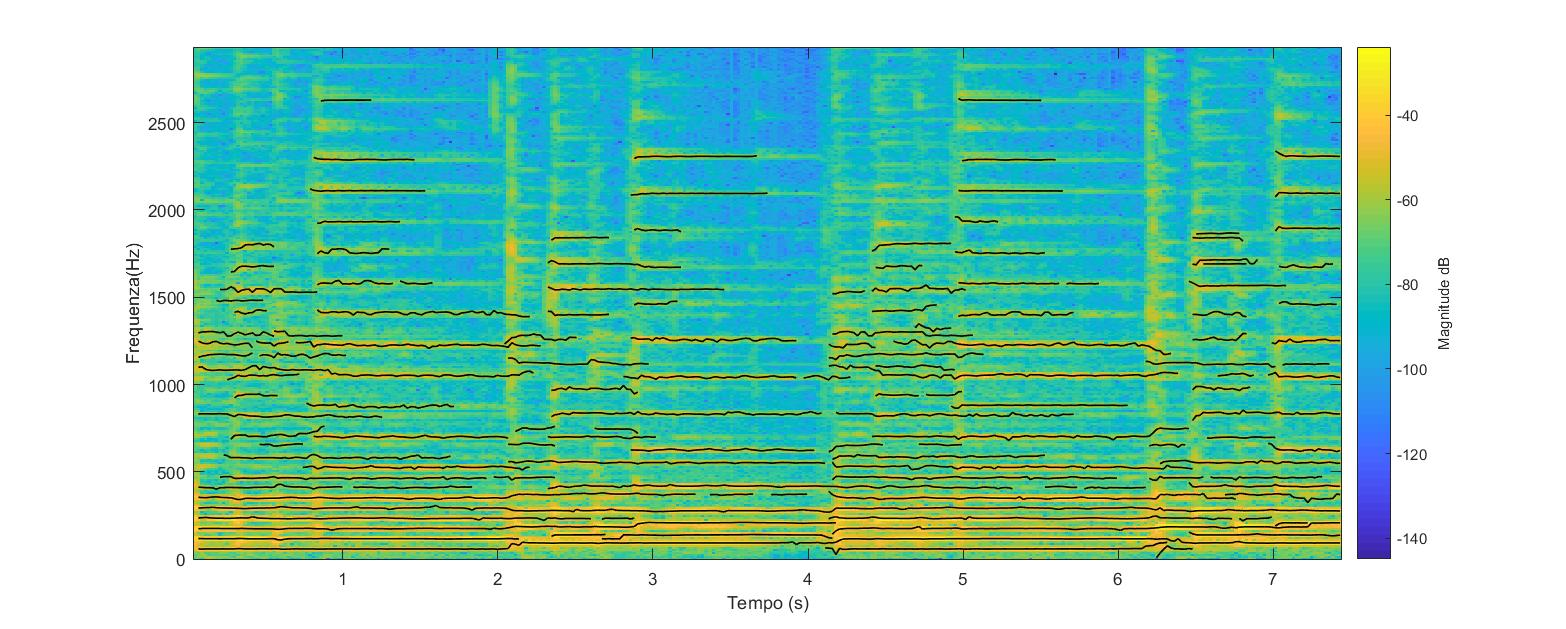
\includegraphics[height=70mm]{img/wither}}
\caption{Spettrogramma con il tracciamento delle singole componenti}
\label{fig:wither}
\end{figure}			

\clearpage

	\section{Analisi timbrica - Rilevamento delle formanti}
	\label{cap3sec3}
		Come si è accennato nel capitolo precedente (Sez. \ref{cap2sec1_1_4}) il timbro è quella caratteristica del suono che permette all'ascoltatore di distinguere due suoni.

In questa sezione si andranno ad estrarre {\itshape feature} che caratterizzano il timbro del segnale, le {\itshape formanti}.
Questa caratteristica oltre ad identificare il suono permette inoltre di valutare le modalità di esecuzione della performance di un musicista, ad esempio la posizione della mano destra o di un plettro durante l'esecuzione di una chitarra elettrica, definendo così un'analisi di equalizzazione generale, utile per definire l'inviluppo spettrale dei due segnali.

Per ottenere le formanti di un segnale, è necessario estrarre dal segnale complesso gli elementi frequenziali che caratterizzano il timbro. Per ottenere queste informazioni si utilizza un modello autoregressivo (AR) lineare {\itshape a soli poli} chiamato Linear Predictive Coding (LPC). Mediante LPC possiamo ottenere una serie di coefficienti $a_k$ (poli di un filtro) e la risposta in frequenza del filtro risultante, corrispondente ad una approssimazione dello spettro del segnale. Tale approssimazione è definita come:

$$  \mbox{\^{x}}[n] = \sum_{k = 1}^{K}a_k x(n-k) $$
dove K è {\itshape l'ordine del filtro}, $a_k$ i coefficienti e $x(n-k)$ i campioni precedenti. Questa formula esprime la combinazione lineare dei campioni precedenti, ovvero l'espressione di un filtro a risposta infinita (IIR - {\itshape Infinite Impulse Response}). \\
L'obiettivo principale della Linear Predictive Coding è l'estrazione dei coefficienti del filtro $a_k$ della funzione di trasferimento definita come:

$$ H(z) = \frac{G}{1 + a_1z^{-1} +\dots+ a_kz^{-k} } $$
Risolvendo il polinomio al denominatore, otteniamo le frequenze dei poli per ogni frame in cui sono stati estratti i coefficienti. Di seguito si illustrano le posizioni dei poli/formanti del segnale di un tratto vocale.

\begin{figure}[htbp]
\centerline{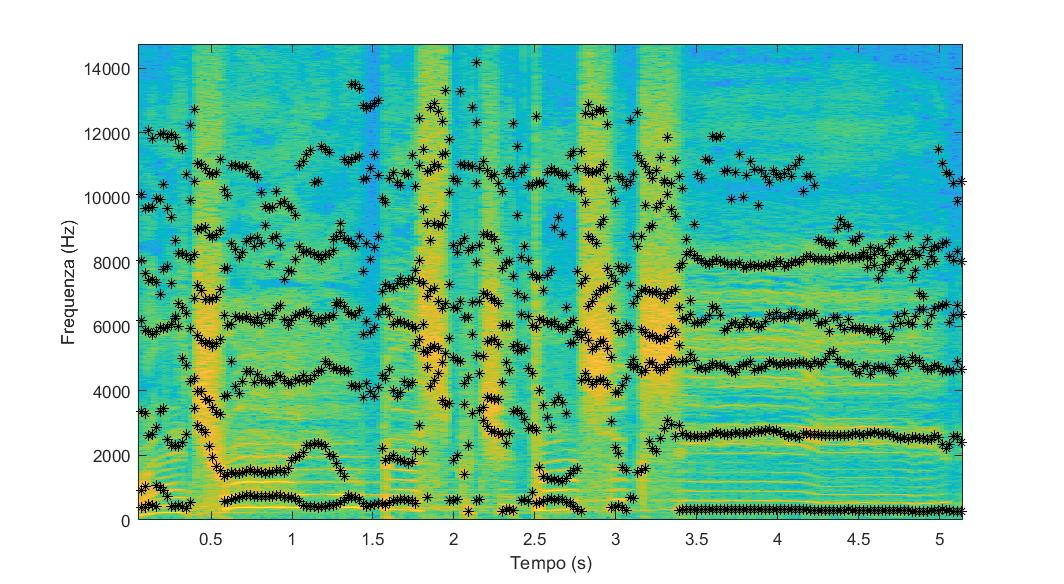
\includegraphics[height=70mm]{img/formant_sono}}
\caption{Poli del modello autoregressivo e il sonogramma del segnale}
\label{fig:formant_sono}
\end{figure}

Infine si rappresenta il risultato ottenuto per un determinato frame del segnale, illustrando il contenuto spettrale, il suo inviluppo e la posizione dei primi sei formanti. Si noti che l'inviluppo ottenuto rappresenta fedelmente il profilo spettrale del segnale.

\begin{figure}[htbp]
\centerline{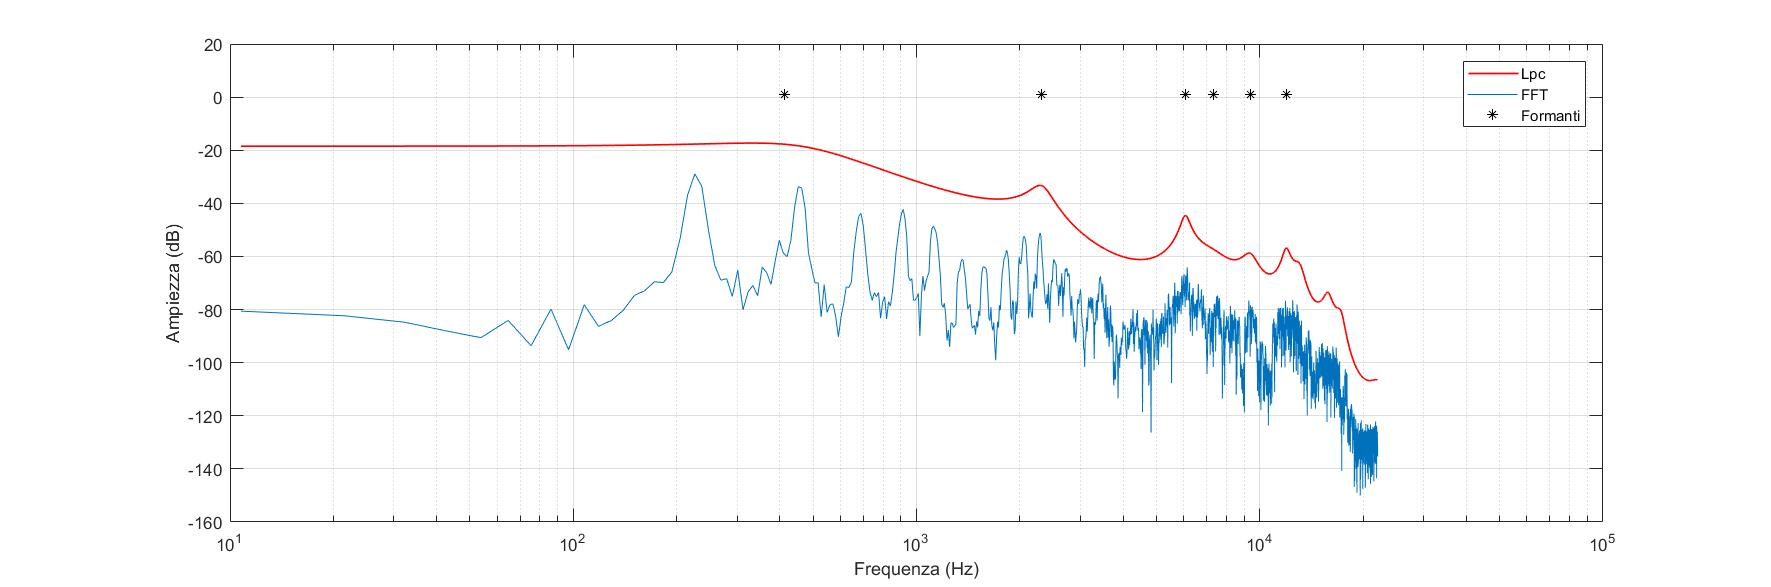
\includegraphics[height=70mm]{img/speech}}
\caption{LPC (Inviluppo spettrale) e la posizione dei formanti in un determinato frame}
\label{fig:speech}
\end{figure}

\clearpage

	\section{Analisi attacco delle note - Onset Detection}
	\label{cap3sec4}
		Un suono, come anticipato nella sezione \ref{cap2sec1_1_1}, ha un inizio e una fine. In questa sezione ci concentreremo in particolare di una caratteristica importante di un evento musicale, ovvero l'istante in cui una nota viene suonata caratterizzandone il transiente di attacco, chiamato mediante il termine inglese {\itshape onset}.\\
{\itshape Transiente}, {\itshape attacco} e {\itshape onset} sono termini che identificano lo stesso concetto ma non hanno lo stesso significato\cite{onset}. La Figura \ref{fig:onset} illustra nel caso più semplice una nota isolata identificando i tre termini.

\begin{itemize}
\item L'{\itshape attacco} di una nota è l'intervallo di tempo nel quale il suono da intensità nulla arriva al suo massimo valore.
\item I {\itshape transienti} sono brevi intervalli di tempo durante il quale il segnale si evolve rapidamente, ad esempio per segnali acustici, il transiente corrisponde all'intervallo di tempo in cui l'eccitazione viene applicata e poi smorzata/attenuata.
\item L'{\itshape onset} è definito come un istante preciso nel tempo atto a identificare l'inizio di un transitorio di attacco. 
\end{itemize}		

\begin{figure}[htbp]
\centerline{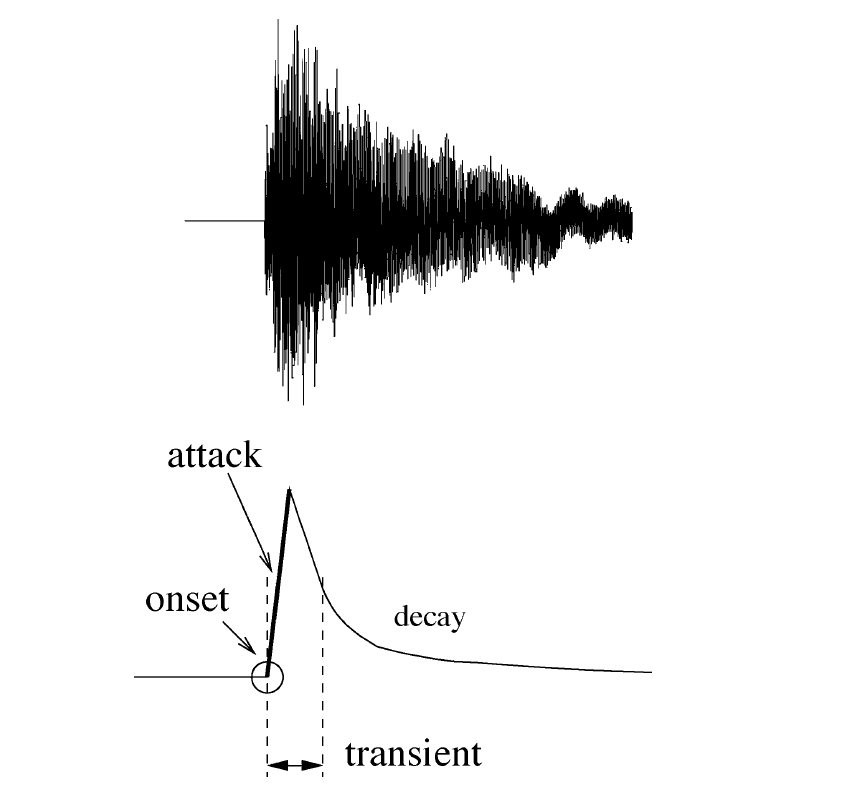
\includegraphics[height=90mm]{img/onset}}
\caption{Attacco, transiente e onset}
\label{fig:onset}
\end{figure}		

La maggior parte dei suoni, durante il transiente di attacco producono un'ampia dispersione di energia a banda larga. Questa situazione si incontra spesso durante la produzione di suoni come colpi di cassa e rullante di una batteria, l'eccitazione di una corda di chitarra mediante un plettro rigido oppure l'emissione vocale in particolar modo l'emissione di consonanti.\\
L'obiettivo è quello di identificare la collocazione temporale dell'{\itshape onset}. Viene implementato l'algoritmo di {\itshape Percussive Feature Detection}.\\

\begin{figure}[htbp]
\centerline{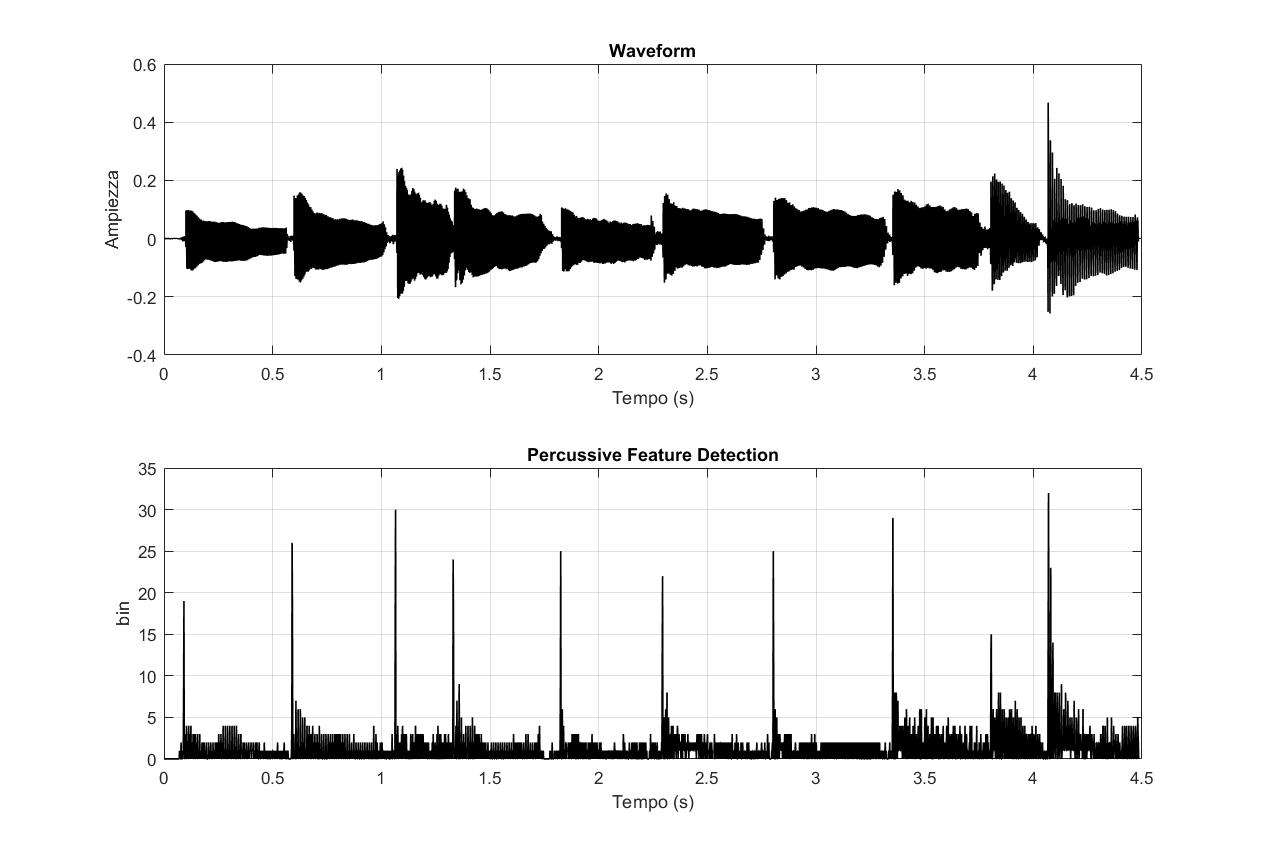
\includegraphics[height=100mm]{img/pfd}}
\caption{Percussive feature detection}
\label{fig:pfd}
\end{figure}

Dopo aver effettuato la STFT sul nostro segnale finestrato mediante una finestra di analisi di lunghezza di 512 campioni\footnote{Un valore basso permette di avere maggior risoluzione temporale ma con lo svantaggio di avere minor risoluzione spettrale}, con un {\itshape hopsize} di 64 campioni (risoluzione temporale di $1.5ms$). Effettuiamo la differenza in {\itshape decibel} tra un frame temporale e quello successivo\cite{pfd} definita come:

$$ X'(k,m) = 20\mbox{log}_{10}\frac{X(k,m-1)}{X(k,m)}$$
dove $X(k,m)$ è la magnitudine al frame $m$ alla frequenza del bin $k$.

Al fine di rilevare la presenza di un onset si definisce la seguente equazione :

$$ 
Pe(m) = \sum_{k = 1}^K \left[
\begin{array}{cc}
P(k,m) = 1 & \mbox{if} \; X'(k,m)>T \\
P(k,m) = 0 & \mbox{otherwise}
\end{array}
\right.
$$

dove T è una soglia che indica l'incremento di energia espressa in dB necessaria per rilevare gli onset. $Pe(m)$ corrisponde ad un contatore che esprime per ogni frame $m$ il numero di bin che superano la soglia: $P(k,m)$ contiene $1$ se la condizione di soglia è soddisfatta, zero altrimenti. Si noti che l'energia reale non è significativa in $Pe$, si esprime solamente la quantità di dispersione a banda larga prodotta dalla percussione del suono. La figura seguente illustra l'approccio effettuato.

L'individuazione della posizione corrispondente all'inizio della nota ora è molto semplice da individuare, fissata una soglia statica per tutta la durata del segnale è possibile estrarre l'informazione temporale necessaria per ogni onset individuato.

	\subsection{Validazione del modello}
	\label{cap3sec4_1}
		Ai fini della validazione del modello implementato si effettua un test mediante due impulsi generati in determinati istanti di tempo, calcolandone le differenze temporali in modo da convalidare la precisione dell'implementazione.
Viene creata una finestra di un secondo dove al suo interno vengono generati due impulsi, il primo (canale {\itshape sinistro}) viene regolarmente generato a metà della finestra ($t_1 = 0.5s$), mentre il secondo(canale {\itshape destro}) viene generato con un ritardo di 1024, 512, 64 campioni, rispettivamente $23.2ms, 11.6ms, 1.5ms$ in modo da valutare la precisione e la risoluzione temporale provocata dalla dimensione della finestra, un ritardo minore avrebbe come risultato una differenza pari a zero, dovuta alla risoluzione minima di 1.5ms.\\
Nella figura \ref{impulsi} si illustra il risultato della {\itshape Percussive Feature Detection} e i risultati ottenuti effettuando la differenza tra le due rilevazioni nella tabella \ref{tab:onset}:
	
\begin{table}[h]
\begin{center}
\begin{tabular}{|c|c|}
\hline
{\bfseries Fig} & Ritardo PFD (ms) \\
\hline
a & 23.2 \\

b & 11.6\\

c & 1.5\\
\hline
\end{tabular}
\end{center}
\caption{Valori di ritardi in relazione alla figura \ref{impulsi}}
\label{tab:onset}
\end{table}

Come si può notare, i valori risultanti del {\itshape Percussive feature detection} coincidono con i ritardi inseriti per la generazione degli impulsi. Questo modello riesce ad analizzare ritardi di 1.5ms, valori più piccoli darebbero come risultato zero perchè il PFD li analizzerebbe come all'interno dello stesso frame di analisi.\\
Una precisione di 1.5ms è una buona risoluzione temporale per analizzare questo tipo di ritardi.

\begin{figure}[htbp] 
\centering 
\subfigure[Impulsi ritardati di 23.2 ms]{ 
	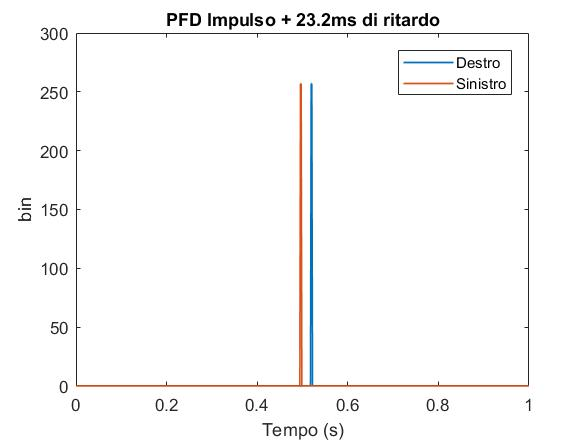
\includegraphics[width=0.45\textwidth]{img/pfd1024}} 
\hspace{7mm} 
\subfigure[Impulsi ritardati di 11.6 ms]{ 
	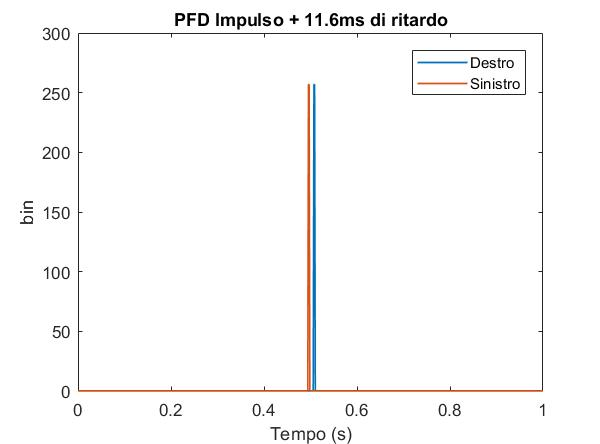
\includegraphics[width=0.45\textwidth]{img/pfd512}} 
\subfigure[Impulsi ritardati di 1.5 ms]{
	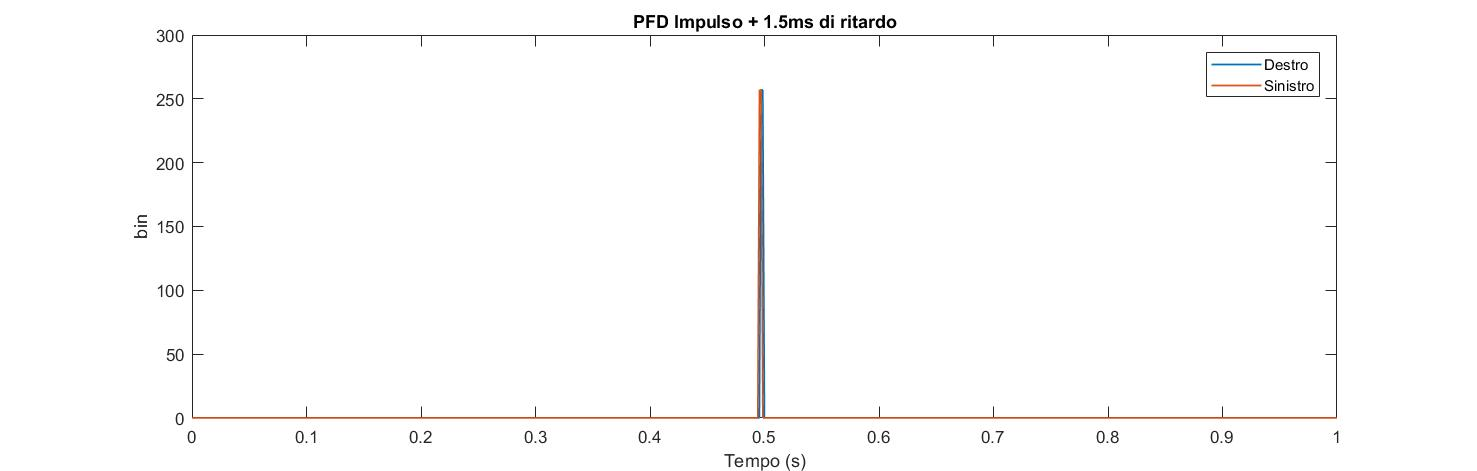
\includegraphics[width=1\textwidth]{img/pfd64a}} 
\caption{Coppie di impulsi ritardati} 
\label{impulsi}
\end{figure}
 
\chapter{Test effettuati e relativi risultati}
\label{cap4}
In questa sezione verranno analizzate le singole coppie incise andando ad estrarre le differenze per ogni {\itshape feature}. Si descriverà il processo di estrazione dei risultati utilizzando come segnale di un riff di chitarra per poi illustrare a fine elaborato una tabella contenente le medie e le deviazioni standard delle differenze per ogni feature in determinati contesti di esecuzione (chitarra e voce).\\

Si prenda come riferimento un riff di chitarra registrato dal sottoscritto di durata di circa $4.5$ secondi. Questo riff è formato da un totale di dieci note singole, estratte dalla scala blues nella tonalità di Sol minore.
Nella figura \ref{fig:wave} si nota che le due forme d'onda non coincidono perfettamente.
Andando ad analizzare le differenze di dinamica dei valori ottenuti, si espongono i seguenti andamenti (Figura \ref{fig:diff_wave}).\\
Il valore medio è illustrato nella tabella che segue:

\begin{table}[h]
\begin{center}
\begin{tabular}{|c|c|c|}
\hline
Feature & Media (dB) & Dev std (dB)\\
\hline
Picco & 2.3935 & 3.9272\\

RMS & 2.2707 & 3.5766\\

Crest Factor & 1.0211 & 1.2891\\
\hline
\end{tabular}
\end{center}
\caption{Valori di media e deviazione standard di Picco, Rms e Crest Factor}
\label{tab:diff_wave}
\end{table}

\begin{figure}[htbp]
\centerline{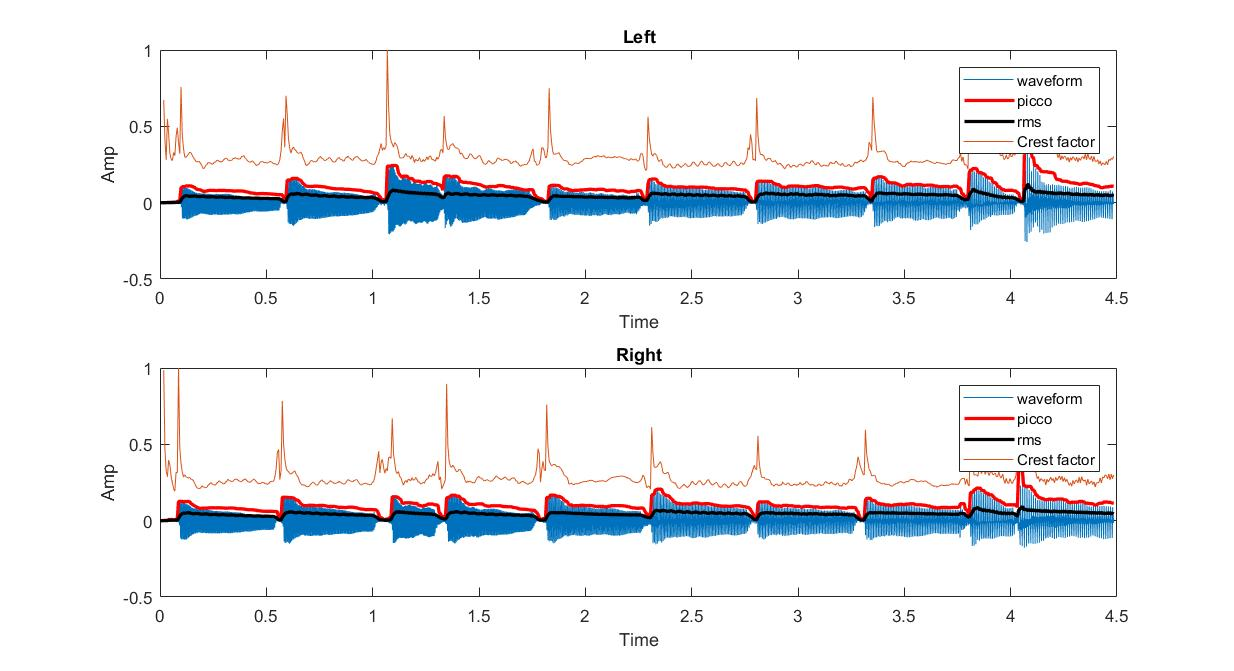
\includegraphics[height=80mm]{img/wave}}
\caption{Forma d'onda di segnali con relativi andamenti di RMS Picco e Crest Factor}
\label{fig:wave}
\end{figure}

\begin{figure}[htbp]
\centerline{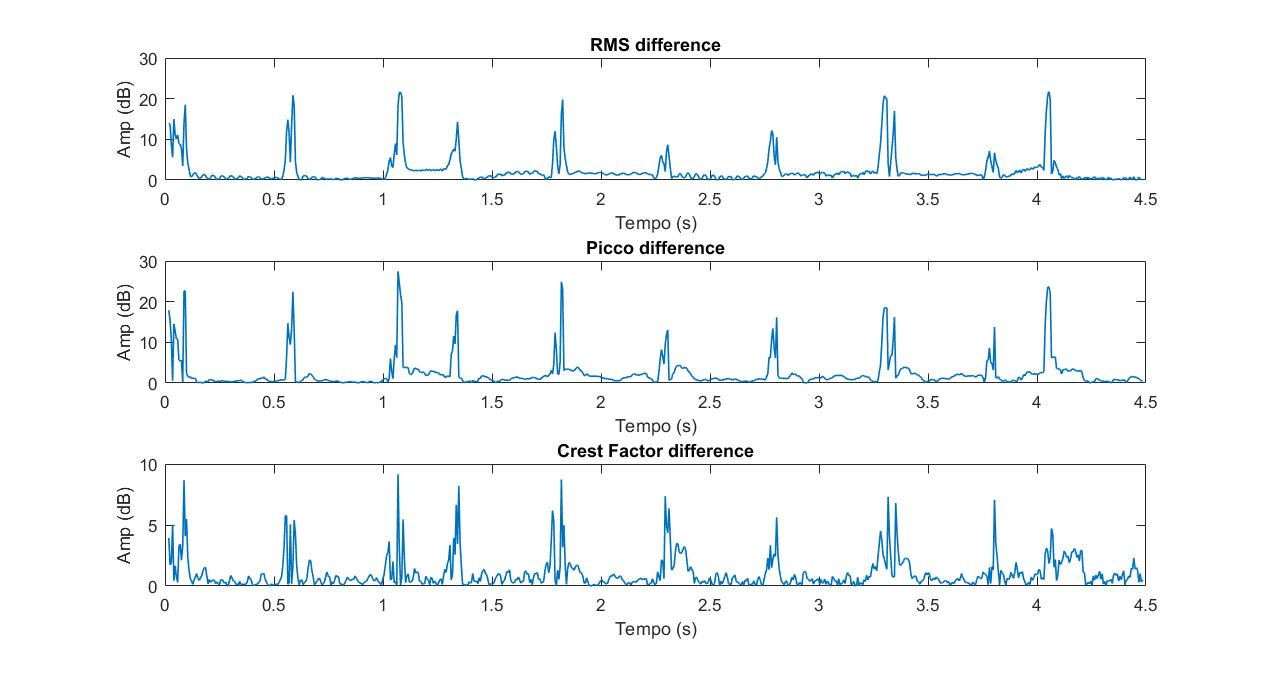
\includegraphics[height=95mm]{img/diff_wave}}
\caption{Differenze di RMS, Picco e Crest Factor}
\label{fig:diff_wave}
\end{figure}

Come si può notare nella figura \ref{fig:diff_wave} le variazioni sono considerevoli al momento in cui la nota viene suonata.

\clearpage

Per quanto riguarda il tracciamento delle armoniche viene preso in esame l'implementazione mediante differenza di fase.
Di seguito si illustrano il tracciamento della fondamentale (rilevata mediante la nota tecnica "{\itshape Cepstrum}") dei due segnali e il tracciamento delle armoniche con le relative differenze.

\begin{figure}[htbp]
\centerline{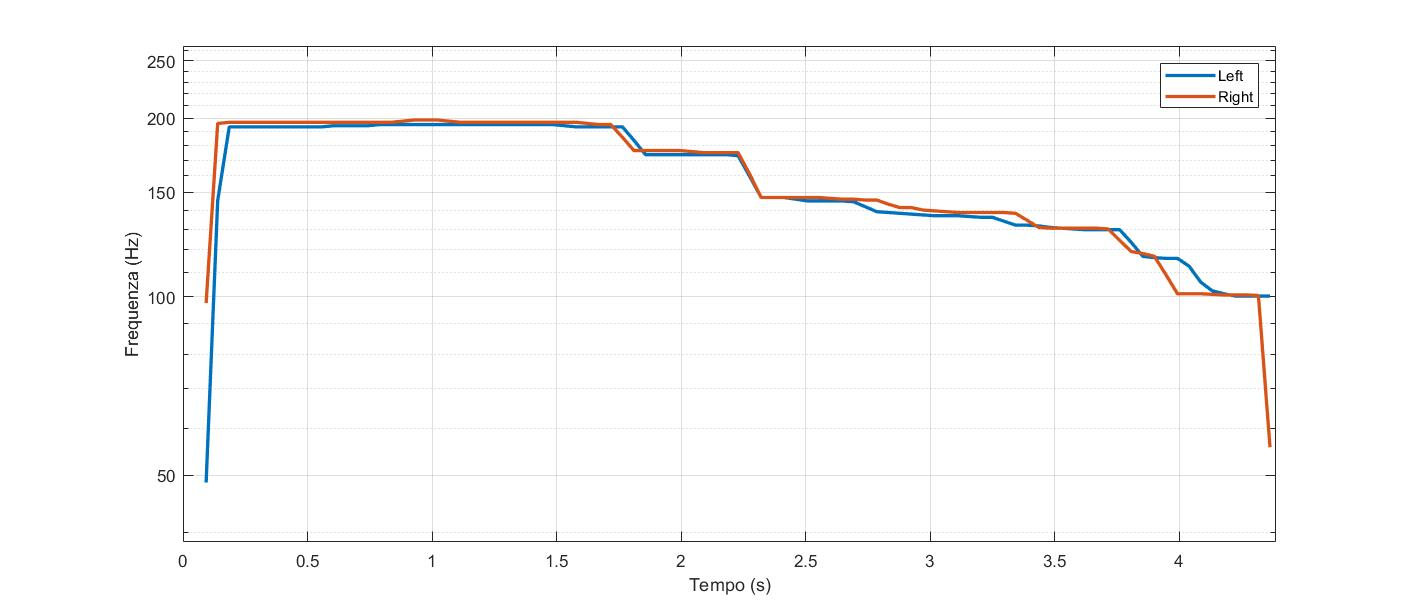
\includegraphics[height=65mm]{img/fond}}
\caption{Rilevamento della fondamentale dei due segnali}
\label{fig:fond}
\end{figure}

\begin{figure}[htbp]
\centerline{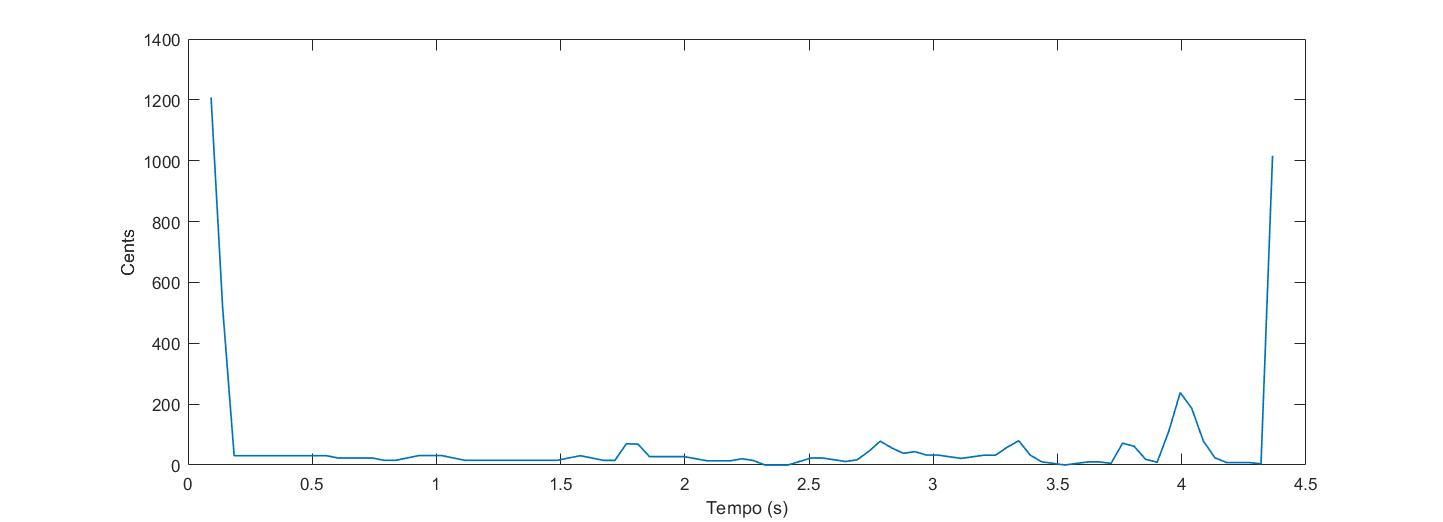
\includegraphics[height=65mm]{img/diff_fond}}
\caption{Variazione in Cent del rapporto tra le due fondamentali}
\label{fig:diff_fond}
\end{figure}

I grafici \ref{fig:fond} e \ref{fig:diff_fond} illustrano che la maggiore deviazione della fondamentale si ottiene quando avviene un cambio di nota.

\clearpage

\begin{table}[htbp]
\begin{center}
\begin{tabular}{|c|c|c|}
\hline
Feature & Media (Cents) & Dev std (Cents)\\
\hline
F0 & 22.9987 & 168.8985\\
\hline
\end{tabular}
\end{center}
\caption{Valori di media e deviazione standard delle variazioni della fondamentale espressi in cent}
\label{tab:diff_fond}
\end{table}
Ora andremo ad esaminare le variazioni delle armoniche tracciate dal modello di analisi. In un segnale complesso è facile avere un tracciamento disturbato da eventuali rumori prodotti da {\itshape ghost note} oppure da vibrazioni emesse dallo strumento stesso o dal musicista. È utile fissare una soglia per individuare i picchi da tracciare, data dal valore di SNR della finestra utilizzata sommata a uno scalare in dB aggiunto dall'utente in modo da cercare di evitare sidelobe.

\begin{figure}[htbp]
\centerline{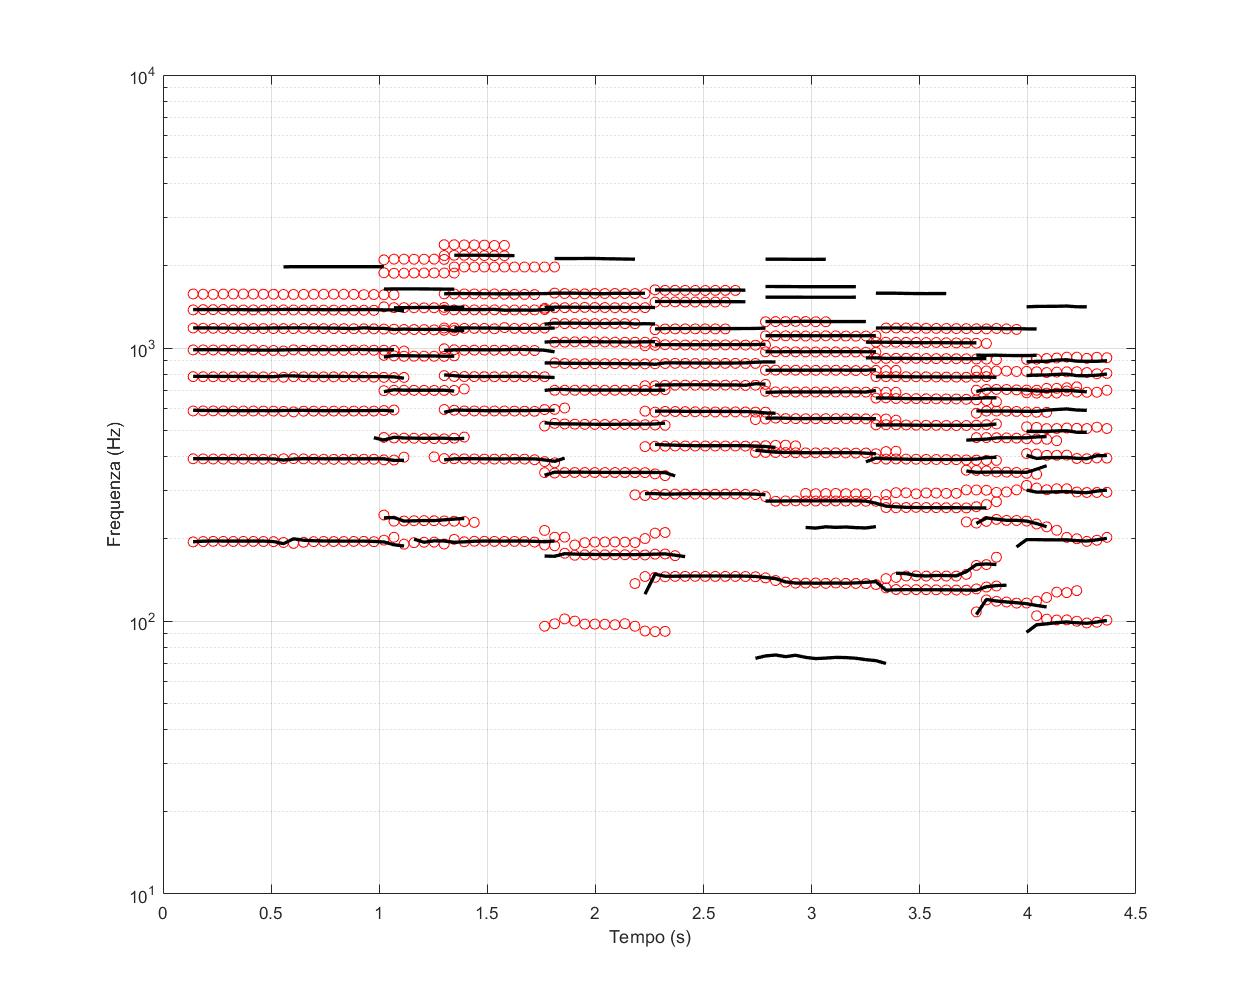
\includegraphics[height=105mm]{img/track}}
\caption{In rosso le armoniche del canale sinistro, in nero quelle del canale destro}
\label{fig:track}
\end{figure}

\clearpage

In figura \ref{fig:track} si illustra in rosso le armoniche del segnale di sinistra, in nero quelle di destra.\\
Sono facilmente individuabili alcuni errori di esecuzione dove introducono artefatti dovuti molto probabilmente ad imprecisione di esecuzione oppure da una soglia di analisi troppo bassa, rilevando così eventuali sidelobe. Infatti è importante selezionare una corretta soglia di analisi in modo da estrarre le differenze per le armoniche che si corrispondono. In questo caso si noti che le prime sette armoniche si corrispondono, di conseguenza si effettuano le differenze di queste armoniche nel primo secondo di segnale e per ognuna  si estrae media e deviazione standard.

\begin{figure}[htbp]
\centerline{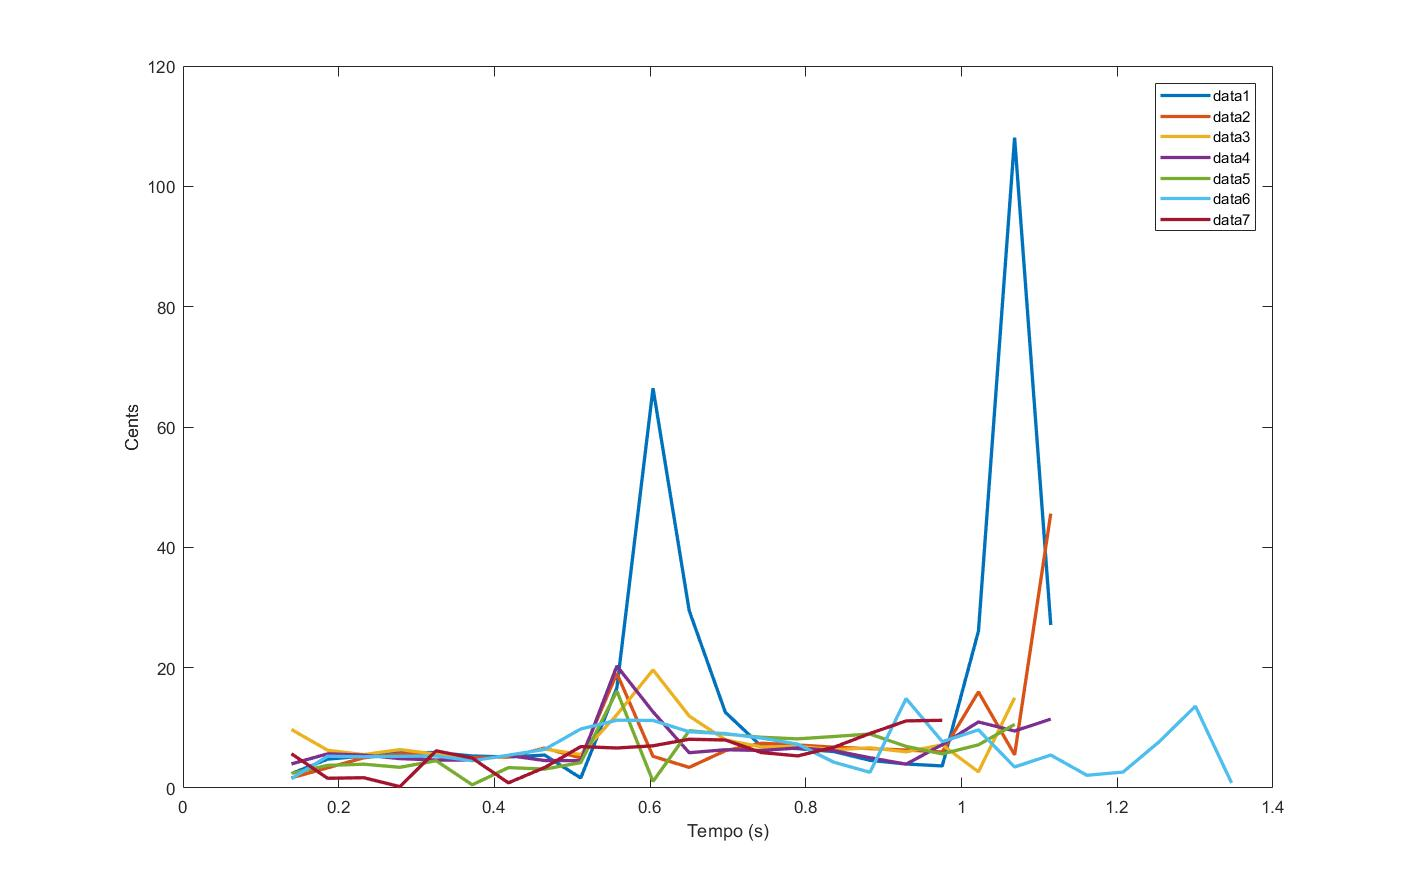
\includegraphics[height=105mm]{img/diff_harm}}
\caption{Variazione in cents delle prime sette armoniche del segnale}
\label{fig:diff_harm}
\end{figure}

Si noti che vi sono dei picchi ({\itshape spyke}) in corrispondenza degli attacchi delle note. Ciò vuol dire che la massima deviazione la incontriamo in corrispondenza di ogni attacco. La minima deviazione, invece, la si incontra tra un attacco e quello successivo, dove la corda si assesta e continua la sua oscillazione.

\clearpage

\begin{table}[htbp]
\begin{center}
\begin{tabular}{|c|c|c|}
\hline
Harm & Media (Cents) & Dev std (Cents)\\
\hline
1 & 16.3649 & 25.1818\\
2 & 8.3804 & 9.1425\\
3 & 1.7743 & 4.1552\\
4 & 7.5003 & 3.8366\\
5 & 5.8884 & 3.8492\\
6 & 6.9706 & 3.2110\\
7 & 5.0333 & 3.5714\\
\hline
\end{tabular}
\end{center}
\caption{Valori di media e deviazione standard delle variazioni delle prime sette armoniche espressi in cent}
\label{tab:diff_harm}
\end{table}
Di conseguenza si calcolano la media e la deviazione standard complessiva delle variazioni delle singole armoniche in modo da ottenere un valore unico.

\begin{table}[htbp]
\begin{center}
\begin{tabular}{|c|c|}
\hline
Media (Cents) & Dev std (Cents)\\
\hline
8.1769 & 3.7699\\
\hline
\end{tabular}
\end{center}
\caption{Valori di media e deviazione standard complessivi delle variazioni delle armoniche}
\label{tab:harm_mean}
\end{table}

\clearpage

Per il rilevamento delle formanti viene calcolato il valore dell'ordine della Linear predictive coding in modo da evitare overfitting mediante la Minimum Description Length (MDL)\cite{mdl}.\\
Vengono inoltre limitati il numero delle formanti a sei ed estratte le differenze delle posizioni in frequenza delle formanti espressi in cents.
Nella figura \ref{fig:ff} si illustra per ogni incisione il contenuto frequenziale di un determinato frame, il suo inviluppo e la posizione delle formanti nello spettro, mentre nella tabella \ref{tab:ff_mean} si illustra il valore complessivo di deviazione.


\begin{table}[htbp]
\begin{center}
\begin{tabular}{|c|c|c|c|}
\hline
Formanti & Media (Cents) & Dev std (Cents) & Valore Medio (Hz)\\
\hline
1 & 162.8759 & 123.9264 & 429.92\\
2 & 190.7448 & 197.5683 & 1544.33\\
3 & 188.7199 & 192.6671 & 3179.64\\
4 & 146.3777 & 163.0557 & 5781.49\\
5 & 114.2583 & 142.1230 & 8062.51\\
6 & 93.3120 & 101.4009 &  10650.68\\
\hline
\end{tabular}
\end{center}
\caption{Valori di media e deviazione standard delle variazioni delle prime sei formanti nel tempo e il valore medio dell'andamento di una sola formante}
\label{tab:ff}
\end{table}

\begin{table}[htbp]
\begin{center}
\begin{tabular}{|c|c|}
\hline
Media (Cents) & Dev std (Cents)\\
\hline
149.3814 & 39.5651\\
\hline
\end{tabular}
\end{center}
\caption{Valori di media e deviazione standard complessivi delle variazioni delle formanti}
\label{tab:ff_mean}
\end{table}

\begin{figure}[htbp]
\centerline{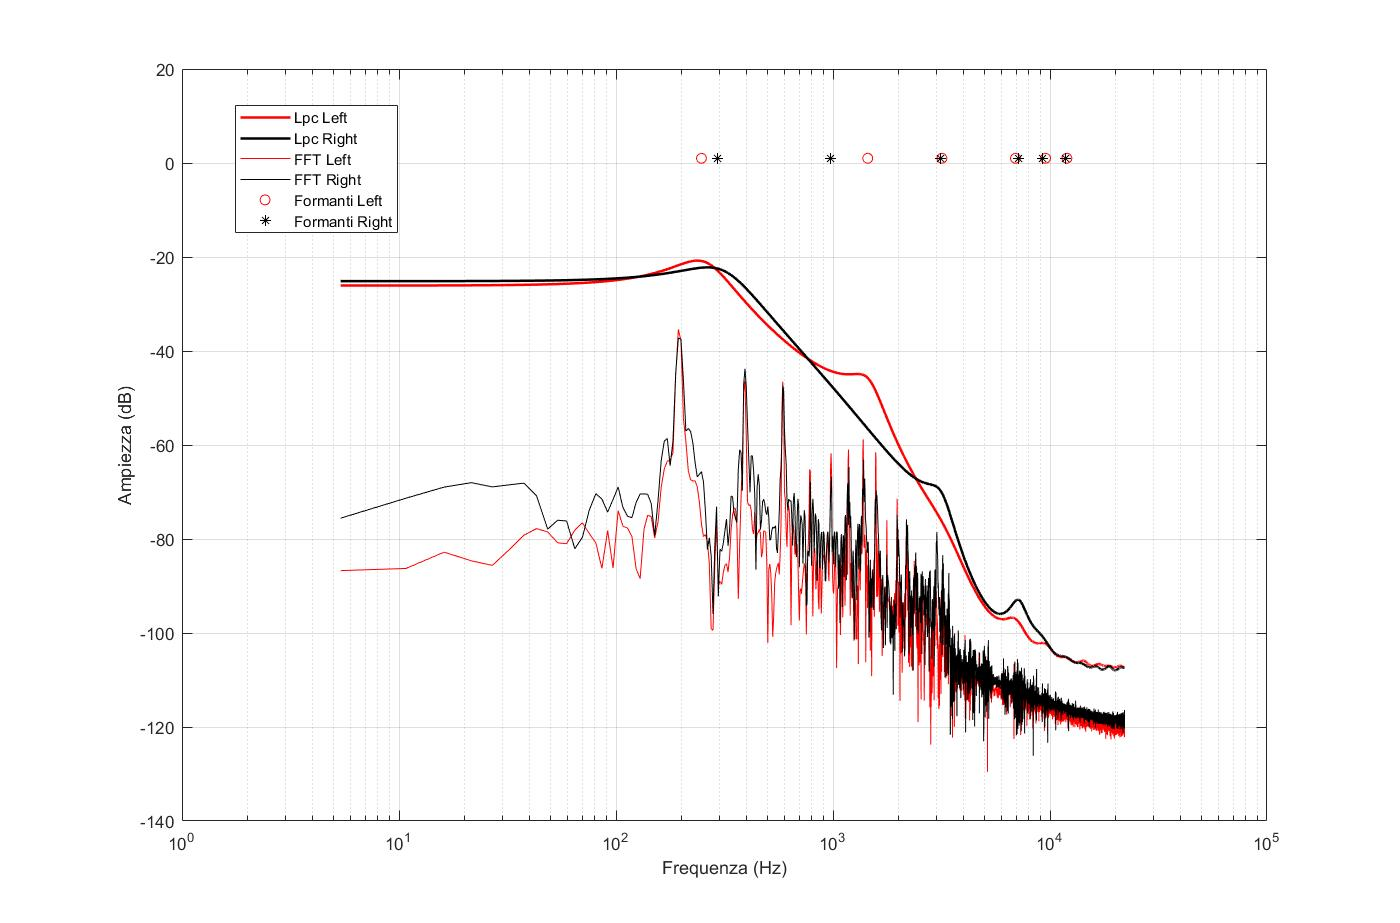
\includegraphics[height=120mm]{img/ff}}
\caption{FFT, Formanti e LPC di entrambi i segnali}
\label{fig:ff}
\end{figure}

\clearpage

Infine come ultima {\itshape feature} vengono estratte le differenze temporali dei due segnali. Di seguito si illustra il risultato ottenuto mediante la Percussive Feature Detection.

\begin{figure}[htbp]
\centerline{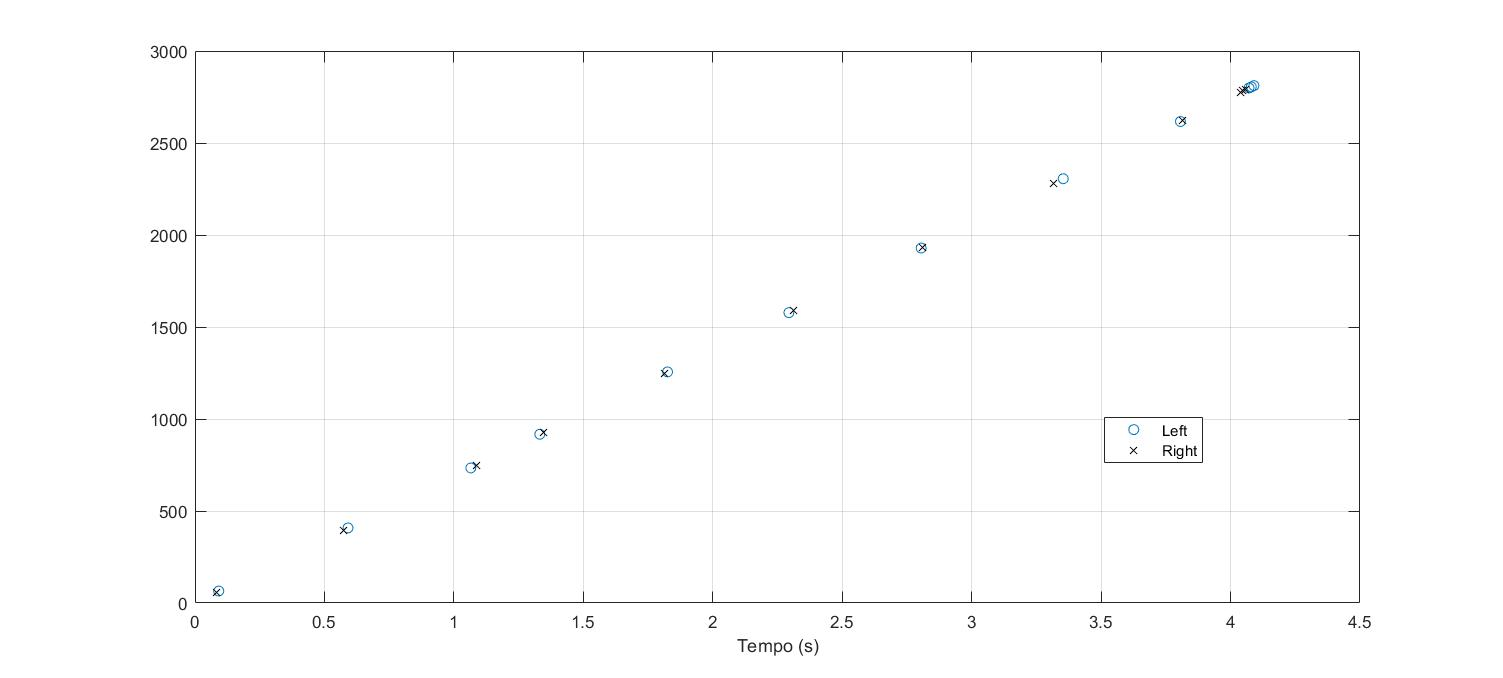
\includegraphics[height=85mm]{img/onset_loc}}
\caption{Posizione nel tempo degli onset}
\label{fig:onset_loc}
\end{figure}

Si noti che ogni onset presenta con il suo doppiato un ritardo/anticipo dovuto all'errore umano nell'esecuzione. Ora avendo localizzato gli attacchi delle note, è possibile estrarre le differenze temporali.

\clearpage

\begin{table}[htbp]
\begin{center}
\begin{tabular}{|c|c|}
\hline
Onset & Ritardi (ms)\\
\hline
1 & 8.7\\
2 & 18.9\\
3 & 21.8\\
4 & 16.0\\
5 & 10.2\\
6 & 16.0\\
7 & 5.8\\
8 & 36.3\\
9 & 7.3\\
\hline
\end{tabular}
\end{center}
\caption{Valori dei singoli ritardi per ogni attacco delle note}
\label{tab:delay}
\end{table}
Calcolando così la media e deviazione standard dei ritardi si estrae un valore unico.

\begin{table}[htbp]
\begin{center}
\begin{tabular}{|c|c|}
\hline
Media (ms) & Dev std (ms)\\
\hline
15.6 & 9.5\\
\hline
\end{tabular}
\end{center}
\caption{Valore di media e deviazione standard complessivo}
\label{tab:rit}
\end{table}

\clearpage

In conclusione, si effettuano i test illustrati per estrarre le variazioni di un dataset contenente dieci riff di chitarra, dieci accordi, per la precisione bicordi di quinta, dieci arpeggi e dieci fraseggi di voce cantata.\\
La doppia incisione viene utilizzata maggiormente per l'incisione di chitarre, per quanto riguarda la voce di solito viene utilizzata per armonizzare la voce principale, di conseguenza viene effettuata l'analisi sulla voce per puro scopo sperimentale.\\

Ogni riff viene sottoposto ad una critica di definizione dove l'ascoltatore dichiara se è presente l'effetto stereofonico desiderato, dopodiche vengono estratti dei fraseggi e analizzati.
Di seguito si illustra una tabella riassuntiva.
Si noti che la variazione della fondamentale non è presente in tutte le modalità di esecuzione, viene effettuata solamente su segnali monofonici dove il metodo Cepstrum utilizzato risulta stabile e affidabile, essa permette un ulteriore controllo sulla variazione frequenziale, mentre teniamo maggiormente in considerazione quello che si è illustrato nei capitoli precedenti.

\begin{table}[htbp]
\begin{center}
\begin{tabular}{|c|c|c|c|c|}
\hline
 & \multicolumn{2}{|c|}{Picco ($dB_{spl}$)} & \multicolumn{2}{|c|}{RMS ($dB_{spl}$)}\\
 & Media & Dev St & Media & Dev St\\
\hline
Riff & 4.59 & 1.94 & 4.23 & 1.87\\
\hline
Accordi & 1.96 & 0.50 & 1.53 & 0.49\\
\hline
Arpeggi & 2,58 & 1.19 & 2.55 & 1.26\\
\hline
Voce & 2,91 & 0.96 & 2.84 & 1.19\\
\hline
\end{tabular}
\end{center}
\caption{Valori complessivi - Media e Deviazione standard}
\label{tab:uno}
\end{table}

\begin{table}[htbp]
\begin{center}
\begin{tabular}{|c|c|c|c|c|c|c|c|c|}
\hline
 & \multicolumn{2}{|c|}{F0 (cent)} & \multicolumn{2}{|c|}{Harm (cent)} & \multicolumn{2}{|c|}{Onset (ms)} & \multicolumn{2}{|c|}{Formanti (cent)}\\
 & Media & Dev St & Media & Dev St & Media & Dev St & Media & Dev St\\
\hline
Riff & 7.23 & 3.63 & 6.47 & 2.76 & 14.63 & 7.21 & 138.51 & 33.35\\
\hline
Accordi & - & - & 8.15 & 8.35 & 12.47 & 8.24 & 100.03 & 28.07\\
\hline
Arpeggi & - & - & 2.87 & 1.94 & 14.15 & 6.78 & 96.48 & 16.70\\
\hline
Voce & 6.40 & 2.01 & 5.65 & 2.11 & 19.08 & 8.59 & 115.53 & 44.54\\
\hline
\end{tabular}
\end{center}
\caption{Valori complessivi - Media e Deviazione standard}
\label{tab:due}
\end{table}

\chapter{Conclusioni e sviluppi futuri}
\label{cap5}

	\section{Conclusioni}
	\label{cap5sec1}
	Osservando i risultati esposti nel capitolo precedente possiamo notare che le variazioni sono molto piccole, basti pensare alla variazione media delle armoniche, il valore massimo corrisponde a $8.15$ cent, ovvero 1/12 di semitono secondo il sistema temperato equabile, definendo così statisticamente la variazione media della pressione di un dito su una corda di chitarra oppure la variazione dell'intonazione di un fraseggio vocale. Come allo stesso modo possiamo definire la precisione di un musicista durante gli attacchi di una nota, in particolare l'errore maggiore lo incontriamo sulle voci con un valore di $19.08$ ms, errore dovuto da molteplici fattori come concentrazione, insicurezza, salute. Sono interessanti le variazioni delle formanti dei due segnali, il valore massimo risulta essere, per l'esecuzione dei riff, di $138.51$ cent, ovvero uno scostamento di oltre un semitono, dovuto alla non identica modalità di esecuzione, nel caso di una chitarra, la posizione del plettro sulle corde: se l'eccitazione della corda avviene in prossimità del ponte, il suono risulterà squillante, invece, se l'eccitazione avviene lontano dal ponte, il suono sarà più rotondo e delicato. Questa posizione incide sulla locazione delle formanti nello spettro. Infine, considerando il valore efficace del segnale (RMS), presenta una variazione massima della dinamica di $4.23 dB_{spl}$, dovuta dalla non identica esecuzione durante l'emissione del suono. \\
	
\clearpage

	\section{Sviluppi futuri}
	\label{cap5sec2}
	Durante lo sviluppo di questo elaborato ho creato, mediante i tool di Matlab un'applicazione che raffiguri, attraverso interfaccia grafica con parametri completamente gestibili dagli utenti, il progetto rappresentato in questa tesi. Questa applicazione permette di caricare i file audio interessati, impostare dimensioni di finestre d'analisi, valori di {\itshape overlap} tra finestre, visualizzare determinati frame, modificare soglie e stampare risultati. Di seguito vengono illustrate varie immagini.\\
Attualmente l'applicazione è in fase di completamento, appena il lavoro sarà ultimato, verrà condiviso apertamente su GitHub (https://github.com/) in collaborazione con il progetto Laboratorio di Informatica Musicale(LIM) (https://github.com/LIMUNIMI).

\begin{figure}[htbp] 
\centering 
\subfigure{ 
	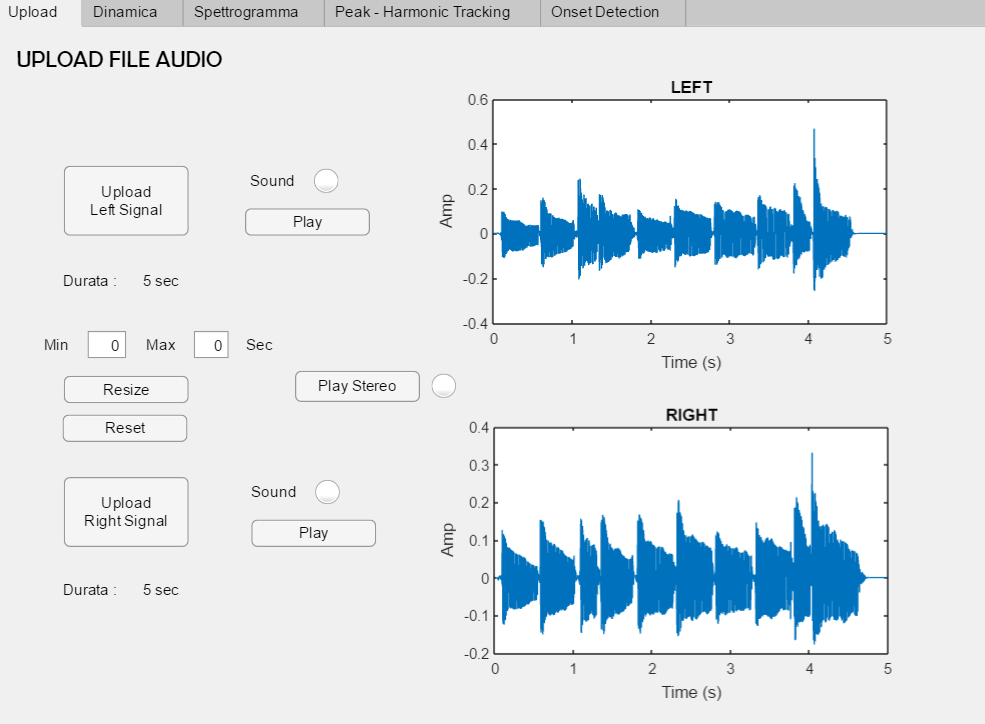
\includegraphics[width=0.55\textwidth]{img/front}} 
\hspace{7mm} 
\subfigure{ 
	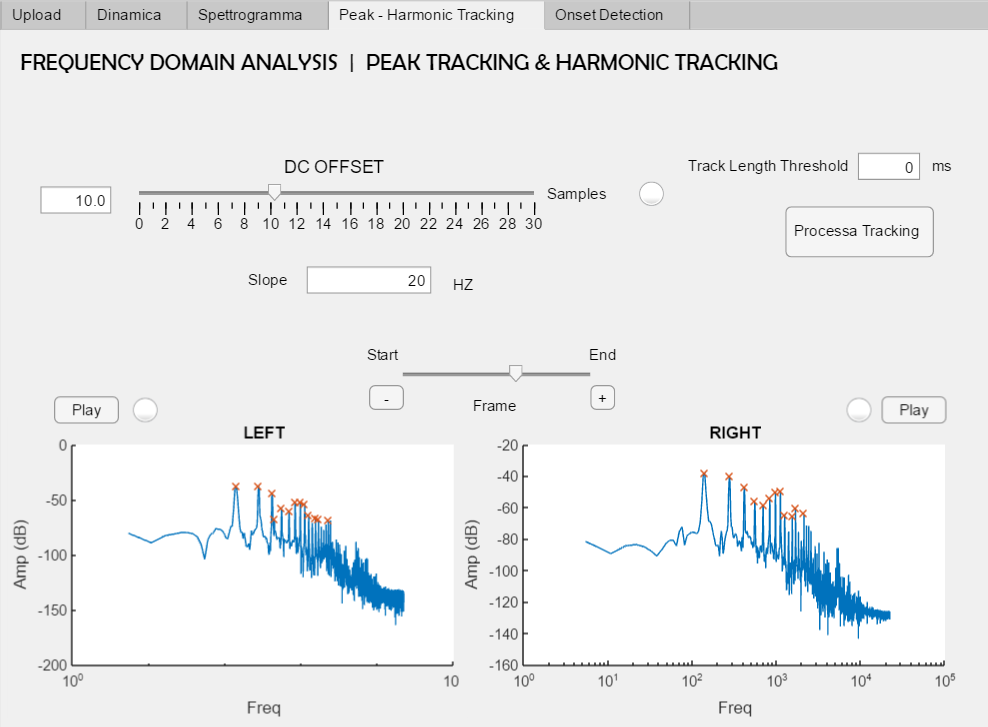
\includegraphics[width=0.55\textwidth]{img/tracking}} 
\subfigure{
	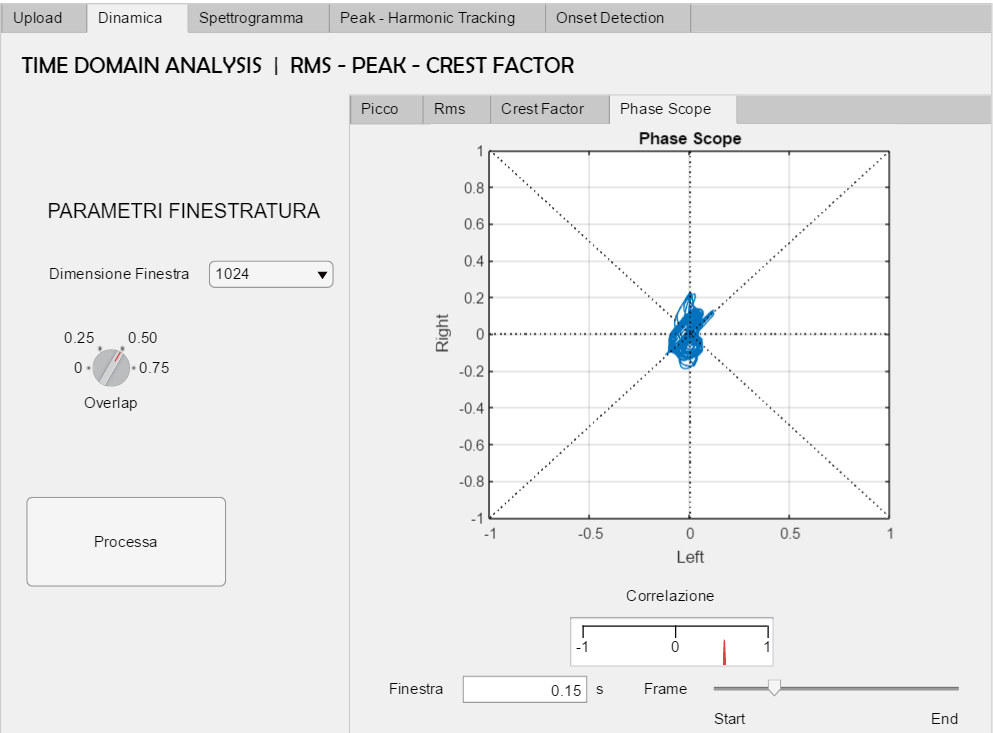
\includegraphics[width=0.65\textwidth]{img/phasescope}} 
\caption{Applicazione in fase di completamnto} 
\label{app}
\end{figure}

\begin{thebibliography}{00}

\bibitem{J_R_Pierce}
J. R. Pierce, {\itshape La Scienza del Suono}, Zanichelli, 1988.

\bibitem{parshl}
Julius O. Smith III, Xavier Sierra, {\itshape PARSHL: An Analysis/Synthesis Program fon Non-Harmonic Sounds Based on a Sinusoidal Representation}, Stanford University, California, 1987.

\bibitem{phase1}
J. L. Flanagan \& M. Golden, {\itshape "Phase Vocoder", Bell System Technical Journal}, vol.45 pp. 1493-1509, 1966.

\bibitem{phasediff}
Karin Dressler, {\itshape Sinusoidal Extraction using an Efficient Implementation of a Multi-Resolution FFT}, Fraunhofer Institute for Digital Media Technology, Ilmenau, Germany, 2006. 

\bibitem{pitch}
De La Cuadra, Patricio, Aaron Master \& Craig Sapp. {\itshape Efficient pitch detection techniques for interactive music}. Proceedings of the 2001 International Computer Music Conference, 2001.

\bibitem{mdl}
Goffredo Haus, Luca A. Ludovico, Giorgio Presti, {\itshape Automatic Annotation of Timbre Variation for Musical Instruments},Proc. of the 13th International Symposium on CMMR, Matosinhos, Portugal, Sept. 25-28, 2017.

\bibitem{lpc}
Amol R. Madane, Zalak Shah, Raina Shah, Sanket Thakur, {\itshape Speech Compressione Using Linear PRedictive Coding} Proceedings of the International Workshop on Machine Intelligence Research, 2009.

\bibitem{pfd}
Dan Berry, Derry Fitzgerald, Eugene Coyle, Bob Lawlor, {\itshape Drum Source Separation using Percussve Feature Detection and Spectral Modulation}, ISSC, Dublin, 2005.

\bibitem{onset}
Juan Pablo Bello, Laurent Daudet, Samer Abdallah, Mark Brian Sandler, {\itshape a Tutorial on Onset Detection in Music Signal}, IEEE Transactions on Speech and Audio Processing, October, 2005.
\end{thebibliography}
\end{document}


